\documentclass[twoside, openright, a4paper,  UKenglish]{report}
\usepackage[dvipsnames]{xcolor}
\usepackage[UKenglish]{uiomasterfp}
\usepackage{amsmath, listings, graphicx, csquotes, amsfonts, commath}
\usepackage[colorlinks=true, allcolors=black, breaklinks=true]{hyperref}
\usepackage{listings}
\usepackage[scale=0.95]{sourcecodepro}
\definecolor{codebackground}{HTML}{FAFAFA}

% For different listing styles, see: https://tex.stackexchange.com/questions/45711/defining-lstset-parameters-for-multiple-languages
\lstset {
  backgroundcolor=\color{codebackground},
  basicstyle=\ttfamily\small,
  breaklines=true,
  columns=fullflexible,
  commentstyle=\color{ForestGreen},
  xleftmargin=4ex,
  frame=none,
  framexleftmargin=2ex,
  keepspaces,
  keywordstyle=\color{RoyalBlue},
  language=haskell,
  mathescape,
  numberstyle=\tiny,
  showstringspaces=false,
  stringstyle=\color{Maroon},
  tabsize=2
}

\usepackage{caption}
\usepackage{subcaption}
\usepackage[normalem]{ulem}
\usepackage{url}

% Macro for personal comments :)
\usepackage{xcolor}
\newcommand{\forsup}[1]{\textcolor{violet}{\texttt{#1}}\\}

% Pseudocode
\usepackage{algorithm2e}
\SetKwFunction{f}{f}

\usepackage{tikz}

% Avoid automatic indentation
\setlength{\parindent}{0pt}

% For captions
\renewcommand*\contentsname{Contents} % or?

% bib
\usepackage[backend=biber,firstinits=true,doi=false,isbn=false,url=false]{biblatex}
\addbibresource{refs.bib}

\begin{document}

\title{Psnodig: Title WIP}
\subtitle{A tool for converting source code to presentation targets}
\author{Sergey Jakobsen}
\uiomasterfp[program={Informatics: Programming and System Architecture}, binding, colour=blue] % vil egt ha purple for haskell da

% link in text:
%\href{https://www.overleaf.com/learn}{help library}

\pagenumbering{roman}
\tableofcontents
\cleardoublepage

% List of figures
\let\oldchapter\chapter
\lstlistoflistings

\let\chapter\oldchapter 
%\cleardoublepage

% List of figures
\let\oldchapter\chapter
\listoffigures

\let\chapter\oldchapter
\cleardoublepage
\pagenumbering{arabic}


\chapter{Introduction}

Pseudocode is commonly used to provide a description of an algorithm at a suitable level of abstraction. It is meant to work as a comprimise between a low-level implementation in a specific programming language, and a natural language description of a problem solution~\cite{whatIsPseudocode}. \\

An advantage of pseudocode is the lack of standardisation, therefore authors are not tied down to the syntax of any particular programming language. This gives them complete freedom to omit or de-emphasize certain aspects of their algorithms. Consequently, pseudocode is first and foremost aimed to serve as a tool for presentation. \\

Consequently, as pseudocode is not executable, there is no omniscient way to verify its correctness. This can, in turn, lead to accidental inclusion of critical inaccuracies. % especially when working with algorithms one is less acquainted with.
When we write code in IDEs, programming languages are often accompanied by static analysis tools that detect anti-patterns and warn about bad practices~\cite{manyLinters, whatIsALinter}. Psudocode writers, on the other hand, are left to their own devices, as identification of anti-patterns and bad practices generally relies on the existence of established standards. \\

\forsup{- Bør jeg forklare hva en IDE er?}

\section{Motivation}

Correct presentations are important in education where the goal is to teach students concepts they were previously unfamiliar with. At university level, concepts within algorithms and data structures have traditionally proved challenging for undergraduates~\cite{algorithmsAreHard1, algorithmsAreHard2, algorithmsAreHard3}. If their first impression of an algorithm is an incorrect presentation, their path is already hampered. \\

In this thesis we present a tool called \textbf{Psnodig} (pronounced snoo-dee~\footnote{Imagine the \textbf{sn} in \textbfit{snow}, the \textbf{oo} in \textbfit{cool}, and the \textbf{dee} in \textbfit{deep}. The silent \textbf{p} is an ode to the silent p in the word \textbfit{pseudocode}, naturally.}), which allows us to convert source code to other, perhaps less technical presentations. The presentation targets in this thesis are pseudocode and flowcharts. The target audience is people who study or work with algorithms. \\

The positive effect of teaching algorithms with flowcharts as an alternative to traditional code has been researched since at least the 1980's, and is still being researched this decade~\cite{flowchartsAreGood1, flowchartsAreGood2, flowchartsAreGood3}. However, tools for direct conversion from source code to flowcharts does not seem to be widespread. \\

We spend much more time \textit{reading} code than we do writing it~\cite[14]{weReadMoreThanWeCode}. Tools like IDEs and linters can only help us so much when it is the \textit{logic} of our programs that we fail to grasp. We believe that Psnodig can be a valuable tool for authors who want to present their algorithms, as well as students who wish to get a better understanding of them. \\

We aim to promote algorithmic thinking through various forms of representation. We believe that this can aid us to better understand and modify our code, which in turn can lead to more efficient and effective programming practices. By not having to worry about syntactic intricacies, the audience can focus entirely on logic underlying the algorithms. \\

Another key point is that the software that \textit{do} let us convert source code to other representations, are completely independent of each other. Most of them also operate with their own DSL to write source code, which makes them even more unavailable. Psnodig, on the other hand, attempts to centralise all these resources, making it a powerful all-in-one tool for any tranlation of our wishes. \\

\forsup{- Bør jeg forklare hva DSL er?}

\forsup{- Er dette paragrafet for en for ``mystisk'' måte å avslutte subsectionen på? Ettersom jeg ikke forklarer hva jeg mener}

\section{Goals}

The overall goal of this thesis is to construct a tool with the following properties:

\begin{itemize}
    \item \textbf{Presentable}, the user can transition their source code to a different of abstraction.
    \item \textbf{Extensible}, the user can add parsers and code generators to work with Psnodig.
    \item \textbf{Customisable}, the user can manually alter the final result.
    \item \textbf{Executable}, the user can run the source code they have written.
\end{itemize}

\forsup{Dette er første gangen jeg nevner `parser` og `code generator`. Bør jeg referere til Section 2.\_.\_, siden jeg ikke forklarer hva det er?}

% Standard tools traditionally fulfill one or the other. Programming languages, in which we can write programs and test them, do not necessary have the appropriate abstraction level to be understood by students at all levels. Pseudocode, on the other hand, is intentionally not executable, and thus the presented ideas cannot be tested directly. The perk of centralising the resources to a single tool makes the job easier for everyone involved. \\

In chapter 3 we will analyse some tools that perform well in one or more area, but fail to satisfy all four.

\section{Contributions}

The main contribution of this thesis is the Psnodig tool, which facilitates the conversion of executable source code to a number of different variants. This is indented to give people an easy and accessible way to look at their code from a different perspective. By using the Psnodig tool, we aim to help people to spend more time writing meaningful code and less time mastering LaTeX libraries, writing boilerplate code, and worrying about maintaining multiple sources. \\

The Psnodig tool comes with a parser for a simple imperative language we call Gourmet, to serve as a proof of concept. It is also accompanied by multiple code generators, which are able to transform a Psnodig abstract syntax tree (AST) back to Gourmet source code, as well as pseudocode and flowcharts written in LaTeX. The latter two utilise the Algorithm2e and TikZ packages, respectively. \\

To summarise, the contributions include:
\begin{itemize}
    \item Psnodig, a tool for converting code from one representation to another. It also comes with an interpreter which works on the intermediate AST representation, so that we can run our code.
    \item The Gourmet programming language, mainly inspired by Go and Python, as a proof of concept. This includes a parser for converting tokens to an AST, as well as a writer to convert the AST back to Gourmet code.
    \item A writer for presenting ASTs with text based pseudocode, utilising the Algorithm2e package in LaTeX.
    \item A writer for presenting ASTs with flowcharts, utilising the TikZ package, also in LaTeX.
\end{itemize}

\section{Project Source Code}

All the source code from the master thesis can be found on Github.~\footnote{The link is \url{https://github.uio.no/sergeyj/Master}. It is actually divided into two folders: \textbfit{psnodig}, containing the source code for the Psnodig tool, and \textbfit{thesis}, containing the LaTeX source code for this thesis.} (NOTE: Alt ligger fortsatt på uio-githuben. Jeg må få overført det til github.com på et tidspunkt. :smilefjes:).

\chapter{Background}

This chapter will cover key concepts one should be familiar with in order to fully understand the rest of this thesis. We start by providing a definition for pseudocode, before discussing how transpiling works. Lastly, we discuss Haskell as an implementation language. We will round off by looking at Pandoc, a transpiler written in Haskell.

\section{Pseudocode}

Pseudocode is a technique for describing computer programs in a more abstract way than programming languages allow, void of a predefined set of rules. Authors can ignore specific syntax and keywords, and instead put their focus on getting their ideas across. This can make programs easier to understand for both non-programmers and programmers alike, particularly when working with unfamiliar algorithms~\cite{whatIsPseudocode}. \\

Since it does not follow any precise syntax rules, pseudocode is subsequently not executable. This is not a bug, but rather a feature of pseudocode: it is intended for \textit{presenting ideas} of code, not \textit{demonstrating results} of code. As Donald Knuth famously put it, after presenting some algorithm implementations in pseudocode~\cite{famousKnuthQuote}:

\begin{verbatim}
    Beware of bugs in the above code; I have only proved
    it correct, not tried it.
\end{verbatim}

When explaining a solution to a non-technical audience, it makes more sense to use pseudocode than source code. More specifically, pseudocode that encapsulates the program's core functionality, to provide clarity on its essential aspects. This enables even individuals without a programming background to provide feedback, based on their understanding of both the problem and now also the proposed solution. \\

Now, since pseudocode has many faces, we must define what we really mean when we refer to pseudocode in the coming sections. In the context of this thesis, we believe that pseudocode can work as an umbrella term for both traditional pseudocode flowcharts.

\subsection{Traditional Pseudocode}

The most conventional form of pseudocode, commonly found in text books on algorithms, published papers, as well as design documents discussing problems~\cite{pseudocodeInBook1, pseudocodeInBook2, pseudocodeInPaper1, pseudocodeInPaper2}. It is also the form that most closely resembles source code, given that it usually includes line numbers, assign statements, and generally presents the problem solution in an imperative matter~\cite[247]{pseudocodeTendsToBeImperative}. \\

Since there is no formal set of rules commanding how pseudocode should look, we are prone to viewing different variations of the same algorithms across different literatures. A frequently presented algorithm is \textbf{Binary search}, a search algorithm that finds the position of a target value within a sorted array. If the target value is not found, some sort of default value is usually returned~\cite{pseudocodeInBook1}. \\

In a note made for the Algorithmic Problem Solving course at the University of Waterloo, professor Naomi Nishimura presented four different variants of the Binary Search algorithm, all written in pseudocode~\cite{differentVersionsOfBinarySearch}. The algorithms are written with a total interval of 26 years from the oldest to the newest. \\

The oldest variant is from 1974, presented in The Design and Analysis of Computer Algorithms by Aho et al.~\cite[139]{binarySearchSource1}. Roughly 17 years later, Lewis et al. present their own version in Data Structures and Their Algorithms~\cite[182]{binarySearchSource2}. The underlying logic stays much the same, though the approaches and syntaxes are different, as seen in \Cref{Binary Search by Aho et al.} and \Cref{Binary Search by Lewis et al.}, respectively. \\

\begin{lstlisting}[caption={Binary Search by Aho et al.}, captionpos=b, label={Binary Search by Aho et al.}]
procedure SEARCH(a, f, l):
if f $>$ l then return "no"
else
    if a = A[$\lfloor$(f + l)/2$\rfloor$] then return "yes"
    else
        if a < A[$\lfloor$(f + l)/2$\rfloor$] then
            return SEARCH(a, f, $\lfloor$(f + l)/2$\rfloor$ - 1)
        else return SEARCH(a, $\lfloor$(f + l)/2$\rfloor$ + 1, l)
\end{lstlisting}

\begin{lstlisting}[basicstyle=\footnotesize\ttfamily, caption={Binary Search by Lewis et al.}, captionpos=b, label={Binary Search by Lewis et al.}]
function BinarySearchLookUp(key K, table T[0..n-1]): info
{Return information stored with key K in T, or $\Lambda$ if K is not in T}
    Left $\gets$ 0
    Right $\gets$ n - 1
    repeat forever
        if Right < Left then
            return $\Lambda$
        else
            Middle $\gets$ $\lfloor$(Left + Right) / 2$\rfloor$
            if K = Key(T[Middle]) then return Info(T[Middle])
            else if K < Key(T[Middle]) then Right $\gets$ Middle - 1
            else Left $\gets$ Middle + 1
\end{lstlisting}

The wish for automatic generation of pseudocode has been desired for some time, with the intention of presenting ideas without having to worry about the syntax of a particular programming language~\cite{desireToGetPseudocodeGeneration}. Traditional pseudocode allows us to draft ideas in an imperative fashion, the same way we write baking recipes and instructions for building legos. Here, the author is free to omit boilerplate code, include mathematical notation and necessary abstractions, and even resort to natural language where deemed appropriate~\cite{pseudocodeInBook1, freedomOfPseudocode}. \\

As previously mentioned, pseudocode has a well-established history in university curricula. When learning algorithms, data structures, and programming concepts in general, the focus is really on the underlying ideas. The concepts are generally more important than the specifics of how they are implemented in a particular programming language. Thus, the approach of learning with pseudocode prioritises concept comprehension over language-specific knowledge. \\

The usefulness of a tool that converts source code to pseudocode can be backed by a number of factors. For one, existing online translators like Code Kindle.\footnote{Works with C++ and Python, can be found at \url{https://devpost.com/software/code-kindle}. Its source code is also available at \url{https://github.com/Open-Sourced-Olaf/Code-Kindle}.} There also exists research on the topic, that we discuss further in Section 3.3.1. Lastly, there are still being created new styles for dislaying pseudocode~\cite{displayingPseudocode}.

\subsection{Flowcharts}

Flowcharts - in the context of computer science - are a way to model computer programs. Also called flow diagrams, they contain nodes (shapes with text) explaining computational steps, and arrows showing us how the programs proceed. This gives a step-by-step overview of computer programs. \\

Imperative programming languages, like Python, execute their programs line for line. This means that we can almost follow the execution flow by just looking at the order functions are called, and the order of statements within those functions. \\

On the other hand, there are languages with different execution flows. For instance, all processes in a VHDL description are executed concurrently~\cite{vhdl}. In languages with term rewriting, like Maude~\cite{maude}, rewriting rules are applied non-deterministically --- if multiple rules can apply to a term, any one of them may be chosen in an arbitrary order. \\

The imperative way of executing a program opens up for the possibility of converting source code to flowcharts, that still includes text, but also complements it with shapes, arrows and colours. When code stretches over enough lines, it often becomes uniform in appearance and more challenging to comprehend. By contrast, flowcharts explicitly capture the control flow of the program, and makes it possible to direct our focus. \\

Images in computer science is nothing new. One of the most notable examples we have are the ones we use for finite state automata (FSA). An FSA is a machine that either accepts or rejects a given string, by running each symbol through a state sequence uniquely determined by said string. We differentiate betwee deterministic and non-deterministic FSAs, although that is not of importance in our context. What they share, is a number of states, a start state, a transition function and an accept state~\cite{introToAutomataTheory}. \\

\begin{figure}[ht]
    \centering
    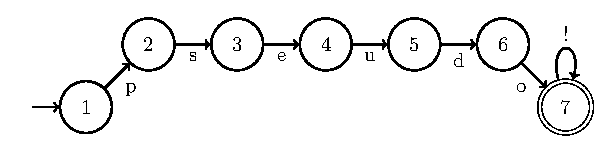
\includegraphics[scale=1.1]{assets/chapter2/Automata.pdf}
    \caption{A finite state automata.}
    \label{An example finite state automata.}
\end{figure}

\Cref{An example finite state automata.} shows an example of an FSA that accepts the word \textbf{pseudo} followed by an arbitrary number of exclamation marks. The FSA has 7 states, and the leftmost arrow indicates that \textbf{1} is the starting state. From here, we can get to the second state if our string starts with the symbol \textbf{p}. Thus, all strings that do not begin with a \textbf{p} are rejected at this point. State 7 has an additional ring within its circle, which means that it is an accepting state. If a combination of symbols have not been rejected at this point, and is finished, it is accepted. \\

State 7 has an arrow leading to itself via the symbol \textbf{!}, meaning that it can end with as many exclamation marks as possible. A string like \textbf{pseudo!!p!!!} is not accepted, however, despite starting with \textbf{pseudo!!} and ending with \textbf{!!!}. Once a string has reached state 7, it can \textit{only} be followed by exclamation marks, or else it is rejected. \\

Warren McCulloch and Walter Pitts were among the first researchers to introduce a concept similar to finite automata, back in 1943~\cite{firstFSA}. Their paper presents a simplified computational model of biological neurons. \\

The first flowcharts in computer science - to the best of our knowledge - were introduced a few years later, by Herman H. Goldstine and John Von Neumann. They used them to depict the flow of programs in ``electronic computing instruments''~\cite{flowchartIn40s}. \\

Also to the best of our knowledge, there does not exist a flourishing amount of research on converting source code to corresponding flowcharts. For instance, when Zhang et al. converted source code to flowcharts for the purpose of plagiarism detection, they used the paid software Visustin~\cite{paperOnPlagiarism}. There \textit{does} exist software to convert source code to flowcharts on the web, like Code2Flow and Mermaid.\footnote{These software are discussed in more detail in Section 3.3.2.} \\

There have been multiple attempts to create flowchart \textit{editors}, most notably by Carlisle et al. and Charntaweekhun et al.~\cite{flowchartEditor1, flowchartEditor2}. These allow us to build flowcharts using the drag-and-drop approach, rather than keeping it all in text form. Benefits of learning with help from visual aid is well documented, and when it comes to computer science, visualisations are especially prominent in the context of machine learning~\cite{ML_Visual1, ML_Visual2, ML_Visual3}. \\

Given the imperative nature of flowcharts, the way they walk through problems step-by-step, it should be no surprise that people have attempted converting flowcharts to pseudocode. Wu et al. has proposed a structure identification algorithm, that can take an identified flowchart as input and automatically generate code in return~\cite{codeFromFlowcharts}. This gives even more ground to perceive flowcharts as (an image based form of) pseudocode. \\

There have been multiple studies documenting the preference for flowcharts when it comes to studying algorithms, already back in the 1980s by Scanlan et al. He recorded how his students overwhelmingly preferred structured flowcharts to pseudocode for comprehending algorithms. Using multiple algorithms of varying complexity, the students most notably indicated that the flowcharts took less time to comprehend, provided fewer errors in understanding, and reduced the number of times they had to look at the algorithms~\cite{flowchartsAreGood1}. \\

More recently, Nita et al. attempted to analyse student's understanding of algorithms with pseudocode and flowcharts. The students were subjected to Algol-like pseudocode and flowcharts. Their conclusion was that the students found it easier to understand the selected algorithms in image format, as compared to a text based approach~\cite{flowchartsAreGood4}.

\subsection{LaTeX}

LaTeX is a document preparation system that is widely used for the production of scientific documents.\footnote{In fact, this thesis is written in LaTeX.} It is an open-source typesetting system recognised for its capabilities in creating visually appealing documents that meet typographic standards. \\

LaTeX operates similarly to traditional programming, as it requires the user to write code to produce a document. The user typesets the document by typing commands in plain text, specifying the structure and styling of the content. This code is then compiled to produce a formatted document, typically in PDF format.\footnote{The concept of compilation is discussed more in-depth in Section 2.3} \\

This is a contrast to more ubiquitous word processors like Microsoft Word or Google Docs, that abide to WYSIWYG principles.\footnote{WYSIWYG is an acronym for \textbfit{What You See Is What You Get}.} This means that they display the final product as it is being edited, and allow users to manipulate the document directly through the GUI. \\

LaTeX builds upon the TeX typesetting system created by Donald Knuth. It has an additional collection of macros that simplifies the use of TeX, and makes it more accessible to non-technical users~\cite[7]{latex}. \\

A distributed collection of macros in LaTeX is called a package. They allow users to add functionality or modify the behaviour of LaTeX, including refining typography, changing the layout of elements, creating graphics and more. In LaTeX documents, they are included using the \texttt{\textbackslash usepackage\{\}} command. \\

As mentioned in Section 1.3, two LaTeX packages are central to  our contributions: \texttt{Algorithm2e} and \texttt{TikZ}. The former is a package to typeset computer programs, whilst the latter, on the other hand, is arguably the most complex and powerful tool to create graphic elements in LaTeX~\cite{algorithm2e, tikz}.\footnote{TikZ was actually used to create the FSA example in \Cref{An example finite state automata.}.}

\subsubsection{Algorithm2e}

After importing the Algorithm2e package, we are free to typeset computer programs within an \textbf{algorithm} environment. \\

There are many macros we can use to typeset our programs. Common ones include \textbf{\textbackslash caption}, to caption our programs, and \textbf{\textbackslash LinesNumbered}, to number the lines of our programs. Each line ends with a semicolon by default, but we can remove them by including \textbf{\textbackslash DontPrintSemicolon}. If we want to add a description of desired input and output above the program, we can do so using \textbf{\textbackslash KwIn\{\}} and \textbf{\textbackslash KwOut\{\}}, respectively. \\

We can define our own keywords by using the \texttt{\textbackslash SetKw\{\}\{\}} macro. If we define \texttt{\textbackslash SetKw\{KwBreak\}\{break\}}, we can add \texttt{\textbackslash KwBreak} to our LaTeX, that is then displayed as \KwBreak in the compiled version. \\

There are also more specific macros, like \texttt{\textbackslash SetKwProg\{Prog\}\{Title\}\{is\}\\\{end\}}. \texttt{Prog} is what we refer to in our LaTeX, \texttt{Title} is what is displayed (like \KwBreak in the previous paragraph), \texttt{is} directly follows \texttt{Title}, and \texttt{end} is the last line of the program. We can write multiple programs within the same \textbf{algorithm} environment. Another common macro is \texttt{\textbackslash SetKwFunction\{f\}\{f\}}. This allows us to write \texttt{\textbackslash f\{arg1, .., arg n\}} in LaTeX, to display \f{arg1, .., arg n} in the compiled version. \\

Algorithm2e comes with multiple predefined English keywords that are commonly found in computer programs, like \textbf{\textbackslash uIf}, \textbf{\textbackslash uElseIf} and \textbf{\textbackslash uElse} for conditionals, and \textbf{\textbackslash While}, \textbf{\textbackslash For} and \textbf{\textbackslash Repeat} for loops.\footnote{The entire documentation can be found here: \url{https://ctan.mirror.garr.it/mirrors/ctan/macros/latex/contrib/algorithm2e/doc/algorithm2e.pdf}.} \\

\begin{figure}[ht]
    \centering
    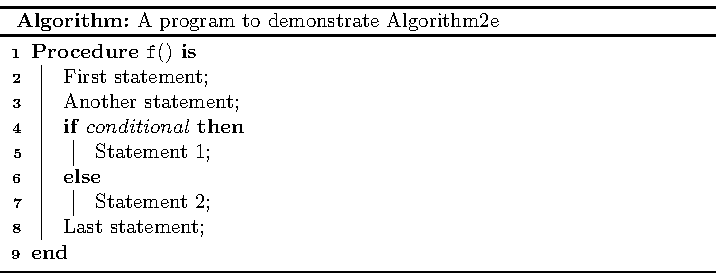
\includegraphics[scale=.95]{assets/chapter2/TheFirstAlgorithm2e.pdf}
    \caption{An example program utilising the Algorithm2e package in LaTeX.}
    \label{The first Algorithm2e program.}
\end{figure}

Since we are still in a LaTeX environment, and backslashes are used for macros in standard LaTeX too, we have to be careful. This is because we are not allowed to rename internal macros. For instance, \texttt{\textbackslash begin} is already a macro in LaTeX, thus attempting to compile a file with \texttt{\textbackslash SetKwFunction\{begin\}\{begin\}} will lead to multiple errors and ruin the compiled result. \\

\subsubsection{TikZ}

As previously stated, TikZ is a powerful tool, and can be used to create just about any graphic element in LaTeX. One of them is flowcharts, which can be constructed using three macros: \texttt{\textbackslash tikzstyle}, \texttt{\textbackslash node}, and \texttt{\textbackslash edge}. \texttt{tikzstyle} lets us define the appearance of nodes and edges, whilst \texttt{node} and \texttt{edge} are used to draw nodes and edges, respectively. \\

\Cref{Rough description of tikzstyle attributes.} gives a rough estimate of how a tikzstyle can be constructed. \\

\begin{lstlisting}[caption={Rough description of tikzstyle attributes.}, captionpos=b, label={Rough description of tikzstyle attributes.}]
\tikzstyle {unique name} =
    [ <shape>
    , minimum width = <x> cm
    , minimum height = <y> cm
    , text <position>
    , draw = <colour>
    , text = <colour'>
    , fill = <colour''>
    ]
\end{lstlisting}

Each tikzstyle has a unique name, so that it can be applied to nodes later on.  The standard shapes are rectangles, but other shapes like diamonds and ellipses can also be imported through libraries. The three colours refer to a node's border-, text- and background colours, respectively. \\

\Cref{How nodes are written with TikZ.} gives a rough estimate of how nodes are written. \\

\begin{lstlisting}[caption={How nodes are written with TikZ.}, captionpos=b, label={How nodes are written with TikZ.}]
\node (unique name)
      [metadata]
      {text displayed on node}
\end{lstlisting}

All nodes should have a unique name, for the purpose of being referenced later. The square brackets denote metadata, like what the node should look like (by referencing a tikzstyle), or the node's positioning relative to other nodes. The curly brackets is the text displayed within the node body. \\

\Cref{How edges are written with TikZ.} shows how most edges are written. It is important to note that nodes must already be defined prior to being referenced by an edge. \\

\begin{lstlisting}[caption={How edges are written with TikZ.}, captionpos=b, label={How edges are written with TikZ.}]
\draw [edge] (node) -- (node')
\end{lstlisting}

\begin{figure}[ht]
    \centering
    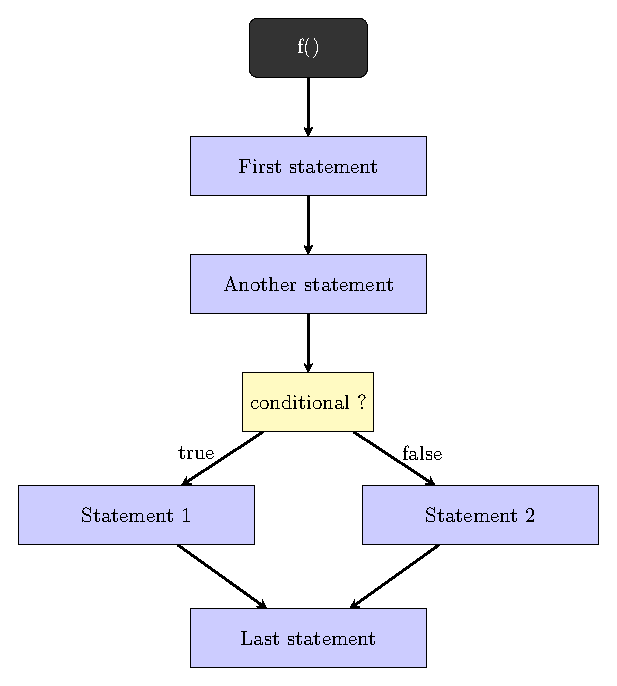
\includegraphics[scale=.9]{assets/chapter2/TheFirstFlowchart.pdf}
    \caption{An example flowchart utilising the TikZ package in LaTeX.}
    \label{The first Flowchart program.}
\end{figure}

\section{Compilers}

A compiler is, in simple terms, a tool that reads a program in a high-level language and translates it to an executable target program. It consists of a frontend and a backend. The frontend is often referred to as the analysis part (analysing the source program before constructing an intermediate representation), whilst the backend is referred to as the synthesis part (patches together the desired target program from that intermediate representation)~\cite{whatIsACompiler}. \\

\begin{figure}[ht]
    \centering
    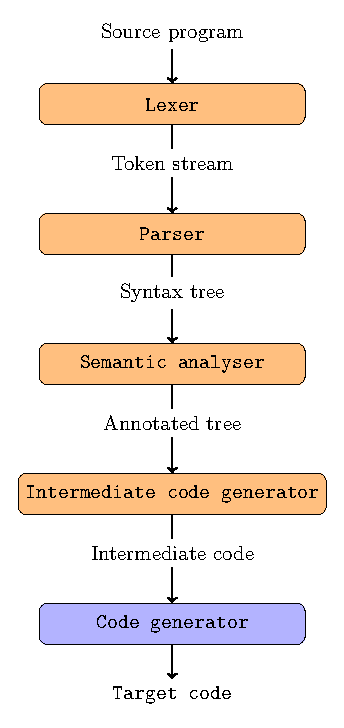
\includegraphics[scale=0.7]{assets/chapter2/PhasesOfCompiler.pdf}
    \caption{The phases of a typical compiler.}
    \label{compilerPhases}
\end{figure}

The frontend of a compiler is responsible for reading the character stream of a source program, and converting them into appropriate tokens. These tokens are then used to create an intermediate representation of the source program. It is during the analysis part that a compiler will detect a program's syntactic errors, if there are any. \\

Often, the analysis part involves a symbol table that maintains information about syntactic entities of the source program. This is passed along with the intermediate representation to the synthesis part, for optimisation reasons. Common entities are bindings and typing. \\

The backend of a compiler is responsible for producing the desired target program from the intermediate representation. This target program is intended to be executable. For instance, source code written in C is compiled down to an executable binary. \\

The typical phases of a compiler is demonstrated in \Cref{compilerPhases}. The orange nodes demonstrate the frontend, whilst the purple node demonstrates the backend. Some compilers also do more work, like optimising the intermediate- or target code, or both.

\subsection{Source-to-Source Compilers}

A transpiler, formally \textbf{source-to-source compiler}, is a tool that converts input source code to output source code, whilst maintaining a similar abstraction level~\cite{whatIsATranspiler}. The first transpiler to our knowledge was developed in 1978 by Intel, with the aim of translating Assembly source code from an 8080/8085 processor to an 8086 processor~\cite{theFirstTranspiler}. \\

JavaScript, the world's most commonly used programming language~\cite{javaScriptIsCommon}, has a rich history of transpilation. As a language in constant development, it faces an issue where not all browsers are always compatible with its newest features. Babel is a transpiler that converts modern JavaScript into a backwards compatible version.\footnote{Babel can be accessed on \url{https://babeljs.io}} According to Nicolini et al., without a transpiler almost 14\% of web users risk facing a JavaScript bug when accessing a website with new JavaScript features~\cite{babelGood}. \\

Not only JavaScript can be transpiled to JavaScript. In fact, the list of other programming languages and tools that can be transpiled to JavaScript is so extensive that it could likely be a thesis topic of its own.\footnote{This overview \url{https://gist.github.com/matthiasak/c3c9c40d0f98ca91def1} provides a list of 320 languages and tools that compile to JavaScript.} However, we can bring forward some notable exambles. \\

Contrary to JavaScript, TypeScript is structurally typed. TypeScript is syntactically a superset of JavaScript, adding a layer of static typing. The primary purpose of these types is to enhance the development experience by catching potential errors during compilation, as well as making the code more maintainable. However, before the code is run, TypeScript is transpiled into plain JavaScript, and the types are stripped away~\cite{TypeScript}. \\

AlaSQL is an open-source SQL database for JavaScript~\cite{alaSQL}. It lets us write SQL within a JavaScript context, i.e. creating tables and performing CRUD operations. \Cref{JavaScript AlaSQL.} shows how we can create a table, populate it with a few Italian football teams, before selecting the ones who meet our criterion. \\

\begin{lstlisting}[caption={JavaScript code to create, populate and select a table with AlaSQL.}, captionpos=b, label={JavaScript AlaSQL.}]
alasql("CREATE TABLE
        teams (name string, points number)");

alasql("INSERT INTO teams
        VALUES ('SSC Napoli', 49),
               ('Salernitana', 15),
               ('Atalanta', 51)");

const topHalf = alasql("SELECT *
                    FROM teams
                    WHERE points < 40
                    ORDER BY points
                    DESC");
\end{lstlisting}

Despite all the commands being written in SQL, the selected table will have a JavaScript value, as seen in \Cref{The value of topHalf} \\

\begin{lstlisting}[caption={The value of topHalf from \Cref{JavaScript AlaSQL.}}, captionpos=b, label={The value of topHalf}]
[
    {
        "name": "Atalanta",
        "points": 51
    },
    {
        "name": "SSC Napoli",
        "points": 49
    }
]
\end{lstlisting}

JavaScript is practically the only Turing-complete programming language that can be used across browsers for web development. Rather than reinventing the wheel, developers have created transpilers to convert programs in their favourite languages to JavaScript. This allows them to write code in their preferred languages, also for web development. Notable examples inlcude GopherJS, Scala.js and Opal, which transpile Go, Scala and Ruby, respectively, to JavaScript. \\

Transpilation is not exclusive to JavaScript, however. It is a common practice in many other programming languages that must interact with or be portable across diverse systems. For instance, the Haskell compiler GHC (Glasgow Haskell Compiler) used to convert the code to C rather than direct native code generation. This enabled Haskell to run on any platform with a C compiler. It also benefitted directly from others' improvements in C code generation~\cite{HaskellToC}. \\

Another example is a transpiler presented by Lunnikiv et. al, where Python is converted to Rust as an intermediate source code step~\cite{PythonToRust}. The paper shows how pre-existing Python implementations that depend on optimised libraries can be semi-automatically transpiled to Rust. This way, the user can keep writing Python whilst simultaneously basking in the glow of Rust's performance optimisation.

\subsection{Parsers and Code Generators}

We mentioned that the frontend of a compiler is tasked with reading source code, and --- given that it is syntactically correct --- building an intermediate representation. The backend of a compiler is tasked with converting that intermediate representation into target code. \\

Having in-depth knowledge about the entire pipeline of a compiler is not necessary to understand the key points of this thesis. Nevertheless, two important aspects of a compiler that \textit{will} be central focus points, are parsers and code generators. Parsers and code generators play a vital role also in a transpiler. In fact, they are all we really need to build a simple transpiler. When the parser has converted the source code to an intermediate representation, the code generator can convert that intermediate representation into a target program. \\

Technically, the parser and the code generator are completely independent from one another. The only thing they must have in common is the ability to read or write the same intermediate representation. There are several advantages to this, like flexibility and modularity. If we want our transpiler to read or write another language, we can just create an additional parser or code generator. When we add a parser, we do not have to do any changes to our code generator, and vice versa, because they work on the same intermediate representation, independent of how the source- and target programs look like. \\

An example of this in practice is the programming language \textbf{Derw}, an ML language mainly inspired by Elm~\cite{derw}. It comes with a single parser (for the Derw language), but multiple code generators (referred to as just generators) that target JavaScript, TypeScript, Elm as well as English and Derw itself. Since it is open source, anyone can fork the repository and add their own code generator, if they so desire. \\

\Cref{LTE in Derw} shows how expressions like \texttt{6 $<=$ 8} are converted from Derw to English. The token \texttt{lessThanOrEqual} has a left- and right pointer, corresponding to the respective integers. These are extracted, and put on each side of the string \texttt{is less than or equal to}.\footnote{The entire English code generator is located at \url{https://github.com/eeue56/derw/blob/main/src/generators/English.derw}} \\

\begin{lstlisting}[caption={The function that converts a \texttt{Less than or equal}-expression in Derw to English.}, captionpos=b, label={LTE in Derw}]
generateLessThanOrEqual: LessThanOrEqual -> string
generateLessThanOrEqual lessThanOrEqual =
    let
        left: string
        left =
            generateExpression lessThanOrEqual.left

        right: string
        right =
            generateExpression lessThanOrEqual.right
    in
        `$\textdollar${left} is less than or equal to $\textdollar${right}`
\end{lstlisting}

\section{Haskell}

As previously mentioned, we opted for the Haskell programming language to implement Psnodig. Knowing the ins and outs of Haskell is not crucial for understanding the thesis. However, there are some aspects of the language that are key to the implementation, which accounts for a large part of the thesis.

\subsection{Data Types}

Haskell lets us create new data types with the \texttt{data} keyword. In reality, types and data types are the same thing, but the \texttt{type} keyword is reserved to make type aliases. For the remainder of the thesis, type and data type will be used interchangeably. \\

A common type in any programming language is the boolean, shown in \Cref{Recreating the Boolean type with Haskell.}. All types have one or more \texttt{value constructors}, that specify the different values a certain type can have. In this case, the Boolean type can have one of two values: \texttt{True} or \texttt{False}. The pipe operator functions as a disjunction~\cite[109]{LYAH}. \\

\begin{lstlisting}[caption={Recreating the Boolean type with Haskell.}, captionpos=b, label={Recreating the Boolean type with Haskell.}]
data Boolean = False | True
\end{lstlisting}

With Haskell, it is straightforward to create our own data types, that can then be used to model ASTs. For instance, we can create a simple calculator language in just a few lines of code, as shown in \Cref{Data types for a calculator language in Haskell.}. From this, we can construct an AST as the one we see in \Cref{An AST constructed with data types presented in}, intended to model the mathematical expression \texttt{1 + 2 - 3}. \\

\begin{lstlisting}[caption={Data types for a calculator language in Haskell.}, captionpos=b, label={Data types for a calculator language in Haskell.}]
data Program = Program Expression

data Expression =
      CompoundExpression Integer Operator Expression
    | IntExpression Integer

data Operator =
      Plus
    | Minus
    | Times
    | Division
\end{lstlisting}

\begin{lstlisting}[caption={An AST constructed with data types presented in \Cref{Data types for a calculator language in Haskell.}}, captionpos=b, label={An AST constructed with data types presented in}]
Program (CompoundExpression 1 Plus
            (CompoundExpression 2 Minus
                (IntExpression 3))
\end{lstlisting}

The calculator language is endlessly expressive within the limits of integers and the operation values we defined. If we wish to expand our operator data type, we only have to add a pipe and the new value name, as seen in \Cref{An extended version of the Operator data type presented in}. \\

\begin{lstlisting}[caption={An extended version of the Operator data type presented in \Cref{Data types for a calculator language in Haskell.}}, captionpos=b, label={An extended version of the Operator data type presented in}]
data Operator =
      Plus
    | Minus
    | Times
    | Division
    | Exponent
\end{lstlisting}

\subsection{Pattern Matching}

Another integral part of Haskell is its strong type system, that allows for clean and efficient pattern matching. This is a very useful method for deconstructing and working with data, and for making decisions based on the data's shape. \\

An example of pattern matching is demonstrated in \Cref{Haskell function converting values of one type to another.}, with a function converting each value of the Operator type (introduced in \Cref{Data types for a calculator language in Haskell.}) to its string equivalent. The function \texttt{convert} takes a value of type Operator as input, and returns a corresponding value of type String. \\

\begin{lstlisting}[caption={Haskell function converting values of one type to another.}, captionpos=b, label={Haskell function converting values of one type to another.}]
convert :: Operator -> String
convert Plus     = "+"
convert Minus    = "-"
convert Times    = "/"
convert Division = "*"
\end{lstlisting}

If the function shown in \Cref{Haskell function converting values of one type to another.} was to work on the extended Operator data type from \Cref{An extended version of the Operator data type presented in}, the compiler would let us know that our pattern matching is non-exhaustive, as there is no case for the \texttt{Exponent} value. This is one of the features that make pattern matching so powerful and safe. For some types though, like \texttt{Integer}, it can be exhausting to define injective functions. \Cref{A rather lazy Haskell.} shows how the underscore symbol can be used to capture all remaining values of a type. \\

\begin{lstlisting}[caption={A rather lazy Haskell function attempting to convert values of type Integer to its string equivalent.}, captionpos=b, label={A rather lazy Haskell.}]
convertInt :: Integer -> String
convertInt 1 = "one"
convertInt 2 = "two"
convertInt _ = "an integer other than one or two"
\end{lstlisting}

\section{Pandoc}

Pandoc is an example of a transpiler written in Haskell, that converts between different markdown formats~\cite{whatIsPandoc}. It includes a Haskell library, as well as a command-line program. It is able to convert documents from 45 source formats to 63 target formats. Additionally, Pandoc is able to convert documents in LaTeX, Groff ms and HTML into PDFs. \\

At its core, Pandoc is really just a specification of Haskell data types. A Pandoc document has the type \texttt{Pandoc Meta [Block]}. The first attribute is \texttt{Meta}, a document's metadata like its title, its author(s), the date it was written and more. The second attribute is a list of \texttt{Block}. A block is a more intricate data type, shown in its entirety in \Cref{Block data type in Pandoc}. \\

\begin{lstlisting}[caption={The \texttt{Block} data type of Pandocs native representation.}, captionpos=b, label={Block data type in Pandoc}]
Plain [Inline]
Para [Inline]
LineBlock [[Inline]]
CodeBlock Attr String
RawBlock Format String
BlockQuote [Block]
OrderedList ListAttributes [[Block]]
BulletList [[Block]]
DefinitionList [([Inline], [[Block]])]
Header Int Attr [Inline]
HorizontalRule
Table [Inline] [Alignment] [Double] [TableCell] [[TableCell]]
Div Attr [Block]
Null
\end{lstlisting}

The modular design of Pandoc means that adding an input format only requires the program to convert \textit{to} this native representation, whilst an output format only needs to convert \textit{from} it. This is much like parsers and code generators of compilers, but as they are much less intricate, the Pandoc documentation refers to them simply as \texttt{readers} and \texttt{writers}. Throughout this thesis, the words \texttt{writer} and \texttt{code generator} will be used interchangeably.\footnote{In reality, traditional code generators do much more than directly translating data types to a target program. In the context of this thesis, however, code generators will not be asked to do much more. This is also a way to acknowledge that the writers we ultimately construct are not fully fledged code generators like the ones we often see in compilers.} \\

Though it must be said, Pandoc cannot always ensure a completely lossless conversion. As the native representation is less expressive than many of the formats it converts between, details are bound to get lost on the way. For instance, LaTeX is a notoriously rich format, much more so than many of its companions in the Pandoc dynasty. However, Pandoc is an excellent interpreter of lightweight markup languages like Markdown, that are more \textit{neutural} by design~\cite{whatIsPandoc}. \\

To demonstrate an example of how Pandoc works, we provide an example of how a Markdown program can be transpiled to LaTeX. \Cref{markdownProgram} is the Markdown program in question, and \Cref{pandocLatex} partly shows the final LaTeX file.\footnote{The final LaTeX document actually comes with 50 more lines of boilerplate generated by Pandoc. However, we can safely remove them, and leave only what we see in \Cref{pandocLatex}. Compiling this and compiling the original result with boilerplate yields the exact same PDF.} \Cref{internalPandoc} also shows its native representation in Haskell. Meta contains title and date, while the list entries in Block are of type Header and Para. \\

\begin{lstlisting}[caption={A program written in Markdown.}, captionpos=b, label={markdownProgram}]
---
title: Programming languages
date: 2023-02-01
---

# Introduction

This is a paragraph about programming languages

\end{lstlisting}

\begin{lstlisting}[caption={The result of transpiling \Cref{markdownProgram} to LaTeX.}, captionpos=b, label={pandocLatex}]
\$\hspace{0pt}$documentclass[]{article}
\title{Programming languages}
\author{}
\date{2023-02-01}

\begin{document}
\maketitle

\section{Introduction}\label{introduction}

This is a paragraph about programming languages

\end{document}
\end{lstlisting}

\begin{lstlisting}[caption={The internal Pandoc AST of \Cref{markdownProgram}.}, captionpos=b, label={internalPandoc}]
Pandoc
    (Meta {unMeta = fromList
        [ ("title", MetaInlines [ Str "Programming"
                                 , Space
                                 , Str "languages"])
        , ("date", MetaInlines [Str "2023-02-01"])
    ]})

    [ Header 1 ("introduction", [], []) [Str "Introduction"]
    , Para [ Str "This", Space, Str "is", Space, Str "a"
           , Space , Str "paragraph", Space, Str "about"
           , Space, Str "programming", Space, Str "languages"
           ]
    ]
\end{lstlisting}

\chapter{Analysis}

In this chapter, we will be doing problem analysis. We will dive deeper into the problem we are addressing, and why we believe it to be a problem in the first place. We also compare source code with our definition of pseudocode, to get a better feel for their differences. Lastly, we will discuss some of the existing approaches, which already solve parts of the problem.

\section{Problem Definition}

Let us outline the problem at hand more concretely. Simply put, we aim to present computer programs at different abstraction levels, whilst maintaining their underlying ideas. The concept is nothing new, but has traditionally been carried out manually by the programmer. We believe there is a benefit in centralising resources and automating the conversion part. \\

There are several use cases where it is useful to display source code in a different light. Mainly in computer science education, where the goal often is to teach students concepts in a programming language agonstic way. It could also be used by researchers to exchange ideas across preferred programming languages. \\

When teaching computed programming at e.g. university level, it is important to distinguish between a student's grasp of computer science topics and their mastering of a particular programming language. Even though a student struggles with the syntax of, say, Go, it does not mean they have an inability to understand the broader concepts. Thus, the teacher can level the playing field by opting for pseudocode when introducing new concepts. \\

Shackelford and LeBlanc Jr. go as far as to say that using pseudocode can ``free students from the myriad of programming language details that annoy and distract attention from the core issue of algorithmic problem solving''~\cite{dislikeProgLang}. This could also apply to researchers who might wish to exchange ideas across different programming languages. \\

On the other hand, flowcharts can offer a visual approach to understanding programming concepts. If a teacher presents their ideas in the form of flowcharts, the classroom can focus on understanding its underlying ideas. If the ideas are presented in source code, students might be distracted by syntactic nuances of the teacher's preferred programming language. \\

In the context of our problem, and the remainder of this thesis, we treat both traditional pseudocode and flowcharts as pseudocode. To make a distinction, we introduce the terms \textbf{Text based pseudocode} (TBP) and \textbf{Image based pseudocode} (IBP).

\section{Comparing Source Code with Pseudocode}

In this section we aim to show how the same computer program can be presented in three different levels of abstraction. The first one will be source code written in a popular programming language, while the latter two will be TBP and IBP. \\

The program in question is a solution to the \texttt{FizzBuzz problem}, commonly presented in entry level interview settings and beginner programming exercises. The input is an integer \texttt{n}, and the output depends on the integer's value: if \texttt{n} is divisible by 3 and 5 we return \texttt{FizzBuzz}, if \texttt{n} is divisible by 3 but not 5 we return \texttt{Fizz}, and if \texttt{n} is divisible by 5 but not 3 we return \texttt{Buzz}. If \texttt{n} is not dividible by either, we simply return \texttt{n}. \\

\Cref{FizzBuzzGo} shows the program written in the Go programming language. \Cref{FizzBuzz with Algorithm2e.} and \Cref{FizzBuzzTikZ.} show the same program, but with TBP and IBP, respectively. \\

The biggest difference between the Go program and the pseudocodes, is that the former contains boilerplate code. For instance, we have to declare which package the file belongs to. In our case, we simply call the package \texttt{fizzbuzz}. We also have to import a package for converting integers to strings, to convert \texttt{n} before returning it in the last case. This is because functions can only have one return type in Go. \\

\begin{lstlisting}[caption={A Go program solving the FizzBuzz problem.}, captionpos=b, label={FizzBuzzGo}]
package fizzbuzz

import "strconv"

func FizzBuzz(n int) string {
    if n%3 == 0 && n%5 == 0 {
        return "FizzBuzz"
    } else if n%3 == 0 {
        return "Fizz"
    } else if n%5 == 0 {
        return "Fizz"
    }
    return strconv.Itoa(n)
}
\end{lstlisting}

The main similarity between the source code and the TBP is that both versions resemble an executable program. People familiar with programming will likely understand the logic conveyed by the pseudocode, even if they have no prior experience with the Algorithm2e library. Both versions present each instruction as sequential lines, and employ common program language syntax like \texttt{else if} and \texttt{return}. \\

One of the differences is how the TBP version has a specific place for describing input and output. With Go, we would either have to them with comments, or leave the users to guess the desired output. \\

Additionally, since TBP is intentionally not executable, we given total control over what we wish to include and exclude. We are free to emphasise particular parts, and also omit non-essential details. This allows us to increase the understanding of our programs more easily. \\

\begin{figure}[ht]
    \centering
    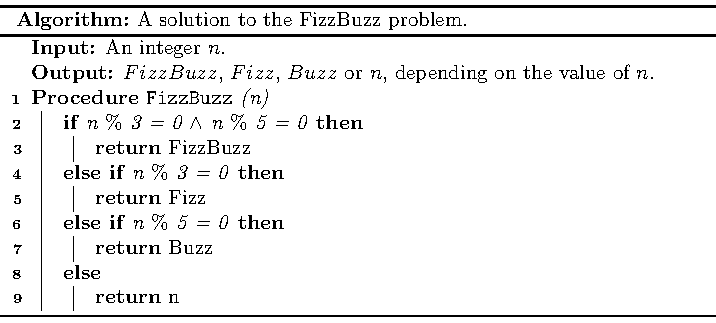
\includegraphics[scale=.95]{assets/chapter3/FizzBuzzAlgorithm2e.pdf}
    \caption{Pseudocode of a program solving the FizzBuzz problem.}
    \label{FizzBuzz with Algorithm2e.}
\end{figure}

All the same can be said for the IBP version, which does not particularly resemble the original source program. In appearance, they are on very different abstraction levels. Whereas the code is written in sequential lines, the flowchart shows colourful shapes wandering off in different directions. \\

The spacing and colourfulness of IBP can make it easier to isolate parts of the program, and to see more precisely how each part works individually. It also makes it easier to follow each path of the program, compared to the Go program, where the order of function calls and scoping of if-statements can confuse even more seasoned programmers. \\

The notation stays much the same, but since flowcharts are not executable, we can again opt for more precise mathematical notation to describe expressions, and exclude static properties like types.

\begin{figure}[ht]
    \centering
    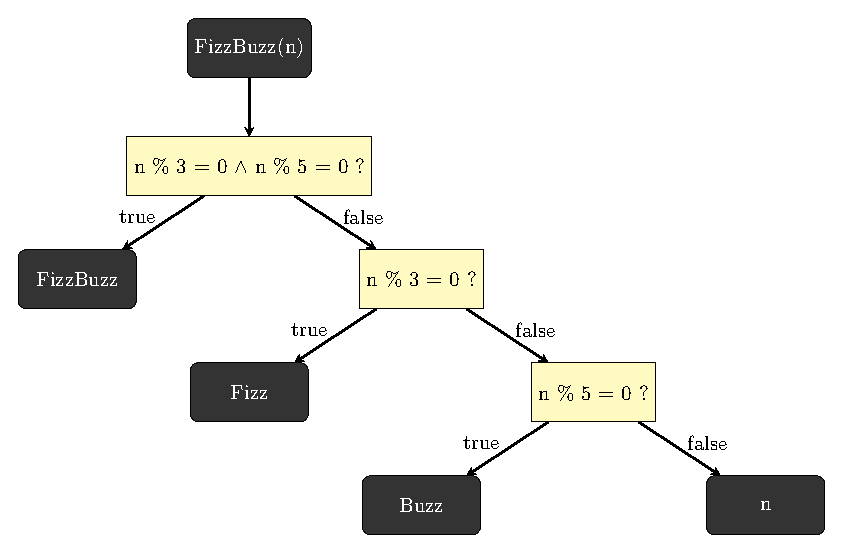
\includegraphics[scale=.75]{assets/chapter3/FizzBuzzTikZ.pdf}
    \caption{Flowchart of a program solving the FizzBuzz problem.}
    \label{FizzBuzzTikZ.}
\end{figure}

\section{Previous work}

This section covers selected works and software that have already solved parts of the problem, in their own right. The first section shows different approaches to convert source code to pseudocode, by applying machine learning. The second section shows interplay between source code and flowcharts, converting one to the other. We also discuss the most basic way of converting between these formats: by doing it manually.

\subsection{Pseudocode}

Despite TBP being used in so many textbooks, online courses and published papers, there are not an overwhelming amount of source code-to-pseudocode editors currently available online. To the best of our knowledge, majority of research on this topic - if not all - centers around machine learning approaches. We will discuss two of these.

\subsubsection{Manual Approach}

The benefits of manually pseudocode manually, is that we are void of any restrictions. We can select the desired abstraction level, we can emphasise what we wish, and the visual formatting is entirely up to us. \\

The biggest downside is the extra effort it requires to maintain two versions of our computer programs. We might change our source code but forget to update the pseudocode. Sometimes we might fail to consistently rename variables, or accidentally misplace parentheses and demonstrate a wrong formula.

\subsubsection{Machine Learning Approach}

To the best of our knowledge, most of the research regarding conversion of source code to pseudocode involves machine learning. Understanding the different machine learning concepts used utilised in these papers is outside the scope of this thesis, but we will give a rough introduction to their main points. \\

In 2015, Oda et al. introduced \textbf{Pseudogen}, a tool for converting Python source code to pseudocode using a statistical machine translation (SMT) approach~\cite{pseudogen}. The pseudocode produced is really a line-for-line description of the Python program provided as input. \\

SMT is a technique to train machine learning models on samples of translations supplied by humans~\cite{whatIsSMT}. It is most commonly used for translating between two natural languages, for instance from English to Italian. In the context of Pseudogen, SMT is used to translate Python to English and Japanese. \\

Despite being a programming language notoriously known for sticking to natural language where many others use more technical notation,\footnote{The best example might be \textbf{\texttt{and}} over \textbf{\texttt{\&\&}}, and \textbf{\texttt{or}} over \textbf{\texttt{||}}, which we find in more or less all other programming languages.} Python still bears the mark of being a programming language. People unfamiliar with programming might still struggle to understand some of the more technical aspects of its syntax, like decorators and closures. \\

\Cref{pseudogenExample1} shows an excerpt taken from the 2015 paper where Pseudogen was first presented. It displays Python source code on the left, and pseudocode on the right. The program in question is an algorithm that solves the \texttt{FizzBuzz} problem, that we also looked at in Section 3.2. \\

\begin{figure}[ht]
    \centering
    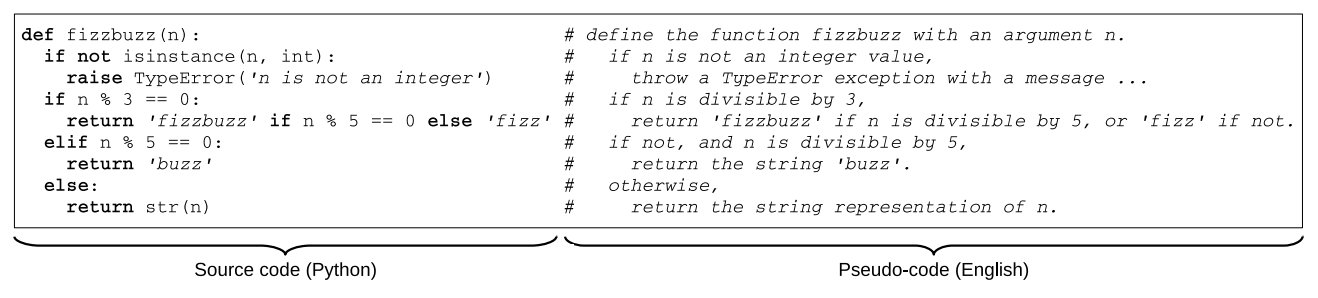
\includegraphics[scale=0.52]{assets/odaetal.png}
    \caption{Python source code translated to pseudocode with Pseudogen. This example is not generated by us, but taken directly from~\cite{pseudogen}.}
    \label{pseudogenExample1}
\end{figure}

Since Pseudogen will translate each line in a servile manner, all error handling is translated too. \Cref{Error handling in Python.} shows some error handling in Python, and \Cref{Error handling in Pseudogen.} shows the result from transpiling it with Pseudogen. The result is considerably more verbose, which defeats some of the point with Python, whose syntax tends to be elegant and succinct, already closely resembling English. \\

\begin{lstlisting}[caption={Error handling in Python.}, captionpos=b, label={Error handling in Python.}]
except ValueError as e:
    print(e)
\end{lstlisting}

\begin{lstlisting}[caption={Pseudocode version of \Cref{Error handling in Python.} generated with Pseudogen. This example is not generated by us, but copied from a video on their website.}, captionpos=b, label={Error handling in Pseudogen.}]
# If ValueError, renamed to e, exception is caught.
    # Call the function print with an argument e.
\end{lstlisting}

Another example is visible in \Cref{listComprehensionPython} and \Cref{listComprehensionPseudogen}, where list comprehension has been translated quite literally. It is plausible to assume people with backgrounds in academia might favour the Python version to the transpiled one, as it closely resembles how we would write set comprehension in mathematics~\cite[11]{setComprehension}. \\

\begin{lstlisting}[caption={A list comprehension of applying f(n) to integers in the range -10 to 10, and placing the results in a list.}, captionpos=b, label={listComprehensionPython}]
a = [f(n) for n in range(-10, 10)]
\end{lstlisting}

\begin{lstlisting}[caption={Pseudocode version of \Cref{listComprehensionPython} generated with Pseudogen. This example is not generated by us, but copied from a video on their website.}, captionpos=b, label={listComprehensionPseudogen}]
# Call the function f with an argument n for every
  n in range of integers from range 10 negative
  integer 10, substitute the result for a
\end{lstlisting}

In 2018, Alhefdhi et al. introduced \textbf{Code2Pseudocode}, a machine learning model which also utilises machine translation techniques. The output follows the format of Pseudogen, but rather than sticking with SMT, they have opted for Neural Machine Translation (NMT). \\

NMT is another variant of machine translation, inspired by neural networks in the human brain. The approach has become the standard for large-scale machine translation, according to a 2019 review and survey carried out by Stahlberg~\cite{nmtOverSmt}. \\

\begin{figure}[ht]
    \centering
    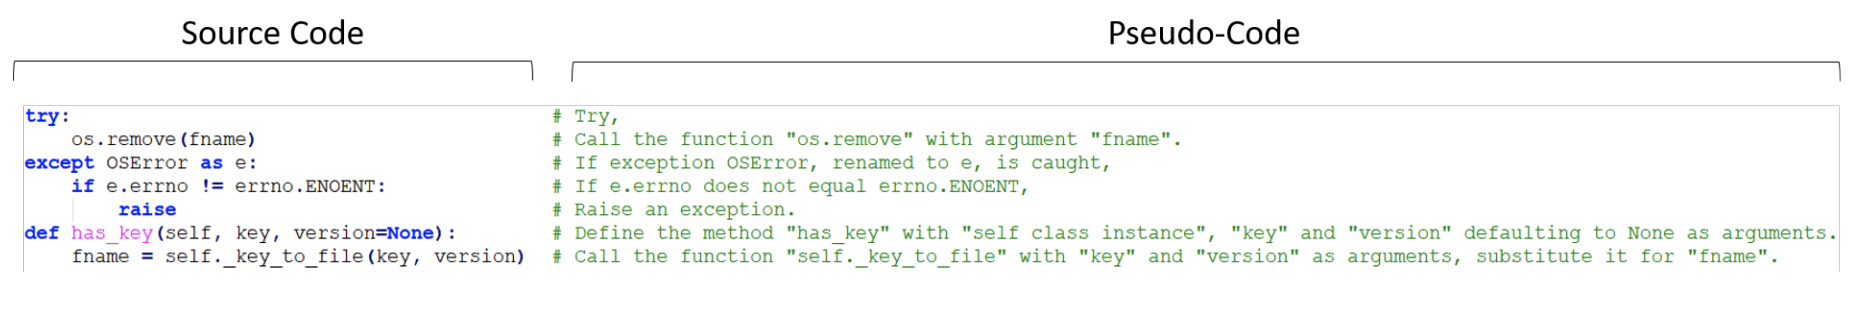
\includegraphics[scale=.37]{assets/chapter3/Code2Pseudocode.png}
    \caption{Python source code translated to pseudocode with Code2Pseudo -code. This example is not generated by us, but taken directly from~\cite{code2pseudocode}.}
    \label{code2Pseudocode}
\end{figure}

\Cref{code2Pseudocode} shows an excerpt taken from the 2018 paper where Code2Pseudocode is presented. It is similar to \Cref{pseudogenExample1} in nature: Python source code on the left, and generated psudocode on the right. The program tries to remove a file from the computer, and raises an error if it fails. \\

Since neither Pseudogen nor Code2Pseudocode have knowledge of Python itself, the descriptions they provide are very general. For instance, the pseudocode in \Cref{pseudogenExample1} does not explain what an ``exception'' is, or what it really means to ``throw an exception''. Likewise, the pseudocode in \Cref{code2Pseudocode} does not tell us that \texttt{os.remove(fname)} will actually remove \texttt{fname} from our computer, only that it calls \texttt{os.remove()} with \texttt{fname} as argument.

%Pseudogen does seem like an excellent tool for translating Python to English, and shows that something like this is indeed possible. However, it is clear that the target audience for its output formats must be people with little to no experience with reading and writing code. Psnodig's intended target audience is somewhat broader, and therefore we believe Pseudogen alone is not enough to solve the problem we are dealing with.

%What the examples in the 2015 paper, as well as a video on their website show,\footnote{The Pseudogen website can be found at \url{https://ahclab.naist.jp/pseudogen/}} is really a line-for-line translation to English. This could be desired in cases where business people on a team are particularly curious about what the product is really doing under the hood (without having to refactor the code base to Cobol). \\

\subsection{Flowcharts}

There is a good deal of research advocating for using flowcharts as an alternative to traditional code when demonstrating computer science concepts~\cite{flowchartsAreGood1, flowchartsAreGood2, flowchartsAreGood3}. Research on ways to construct corresponding flowcharts from source code, however, is not plentiful. \\

In this section we will look at a few different approaches: the naive approach (doing it manually), a flowchart-first approach (writing the flowchart with drag and drop), and a code-first approach (converting programs in domain-specific language to flowcharts).

\subsubsection{Naive Approach}

Yet again, calling it a naive approach might not be entirely accurate, but manually translating our code to flowcharts does introduce some intricacies. For one, like with TBP, we have to maintain both versions, and if we change too much of our main idea, then the time spent on making the IBP version is - to a certain extent - wasted. \\

Another flaw is that we have to spend time thinking about how the flowchart should look like, which parts could and should be abstracted, how they should be presented instead (or if they should be removed altogether) etc. Which colours should the frames have? How should the arrows look? Which font should be used? By automating this process, we do not have to worry about details unrelated to the actual program logic. \\

The perk of doing it this way, however, is that we can do it entirely our way. We can choose which tools we want to use, and if we are already proficient in making flowcharts based on source code, then this actually seems like a natural choice. If we also like spending time on details like colours, fonts, shapes etc., then at least the naive approach does not limit our creativity in any way.

\subsubsection{Flowchart-first Approach}

In 2015, Kosower et al. introduced \textbf{Flowgen}, a flowchart-based documentation framework for C++. The tool converts annotated C++ programs to high-level UML activity diagrams, providing a description of the code's dynamic behaviour~\cite{flowgen}. \\

Flowgen extracts control flow parts of a program, as well as annotations initiated by \texttt{//\$}, to build flowcharts for each function or method. Understanding what C++ programs do is outside the scope of this thesis, with the relevant part being how Flogen represents a program written in executable source code as a flowchart. \\

\Cref{c++prog} shows a C++ program with Flowgen annotations, and \Cref{flowgenExample} shows the corresponding flowchart created by Flogen. We have not generated this flowchart ourselves, instead it is taken directly from~\cite{flowgen}. \\

\begin{lstlisting}[caption={A C++ program.}, captionpos=b, label={c++prog}]
#include \\aux.h''
#include <iostream>
int main()
{
    int control flag=0;
    //$\textdollar$ ask user whether to proceed
    std::cin >> control flag;
    if (control flag==1){
        //$\textdollar$ call shower
        // pointer to the object VINCIA
        VINCIA* vinciaOBJ = new VINCIA();
        vinciaOBJ->shower(); //$\textdollar$
    }
    return 0;
}
\end{lstlisting}

\begin{figure}[ht]
    \centering
    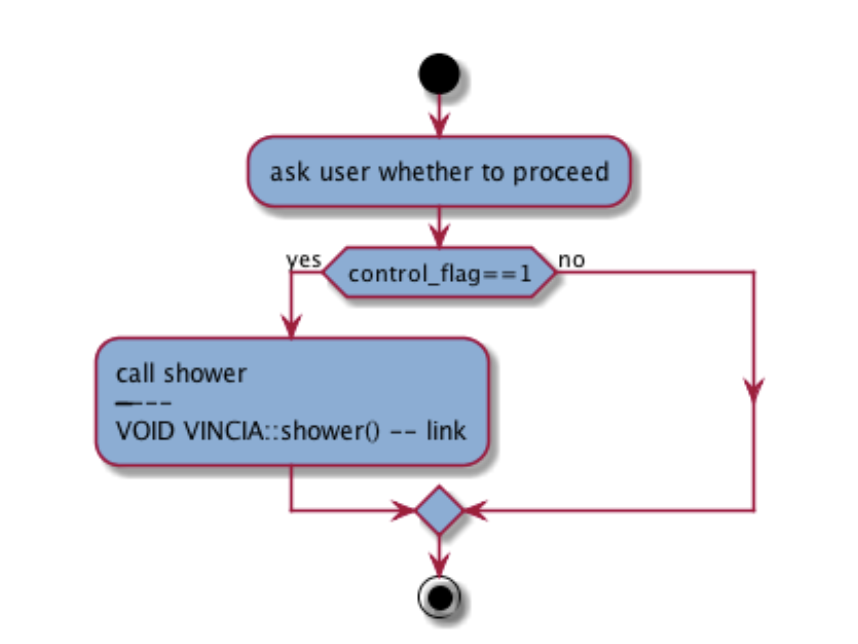
\includegraphics[scale=0.6]{assets/chapter3/Flowgen.png}
    \caption{\Cref{c++prog} converted to a flowchart with Flowgen. This example is not generated by us, but taken directly from~\cite{flowgen}.}
    \label{flowgenExample}
\end{figure}

In 2006, Charntaweekhun and Wangsiripitak propsed a tool that converts flowcharts to an equivalent C program, which is then compiled and executed~\cite{flow2c}. \Cref{flow2cExample} shows an example of converting a flowchart to a C program using their tool, taken from their original 2006 paper. \\

\begin{figure}[ht]
    \centering
    \includegraphics[scale=0.6]{assets/chapter3/bangkok.png}
    \caption{A flowchart converted to an equivalent C++ program. This example is not generated by us, but taken directly from~\cite{flow2c}.}
    \label{flow2cExample}
\end{figure}

\subsubsection{Code-first Approach}

\textbf{Code2Flow} is a tool that lets us create flowcharts with natural language, decorated with a C-inspired syntax. Their website states that we might get away with pasting syntactically correct C programs, but that this is purely incidental. This goes to show that the Code2Flow team have indeed developed a DSL with their own syntax. \\

Flowcharts created with Code2Flow have a few, consistent colours to differentiate parts of their corresponding programs. Start- and end expressions are displayed as red ovals, while all remaining expressions are displayed as blue rectangles. Conditionals, loops and match statements are displayed with red rhombuses, and comments are displayed with orange rectangles. \\

\begin{lstlisting}[caption={A Code2Flow program.}, captionpos=b, label={A Code2Flow program.}]
First statement;
Another statement;
if (conditional) {
  True statement;
} else {
  False statement; // Random comment
}
Last statement;
\end{lstlisting}

\Cref{A Code2Flow program.} shows a program written with Code2Flow, and \Cref{A Code2Flow flowchart.} presents the corresponding flowchart. As we can see, syntactically correct expressions are any combination of UTF-8 characters. Code2Flow will never warn us about syntactic errors, and will \textit{always} try to construct whatever flowchart it can. In turn, there is no clear way to test a Code2Flow program. \\

\begin{figure}[ht]
    \centering
    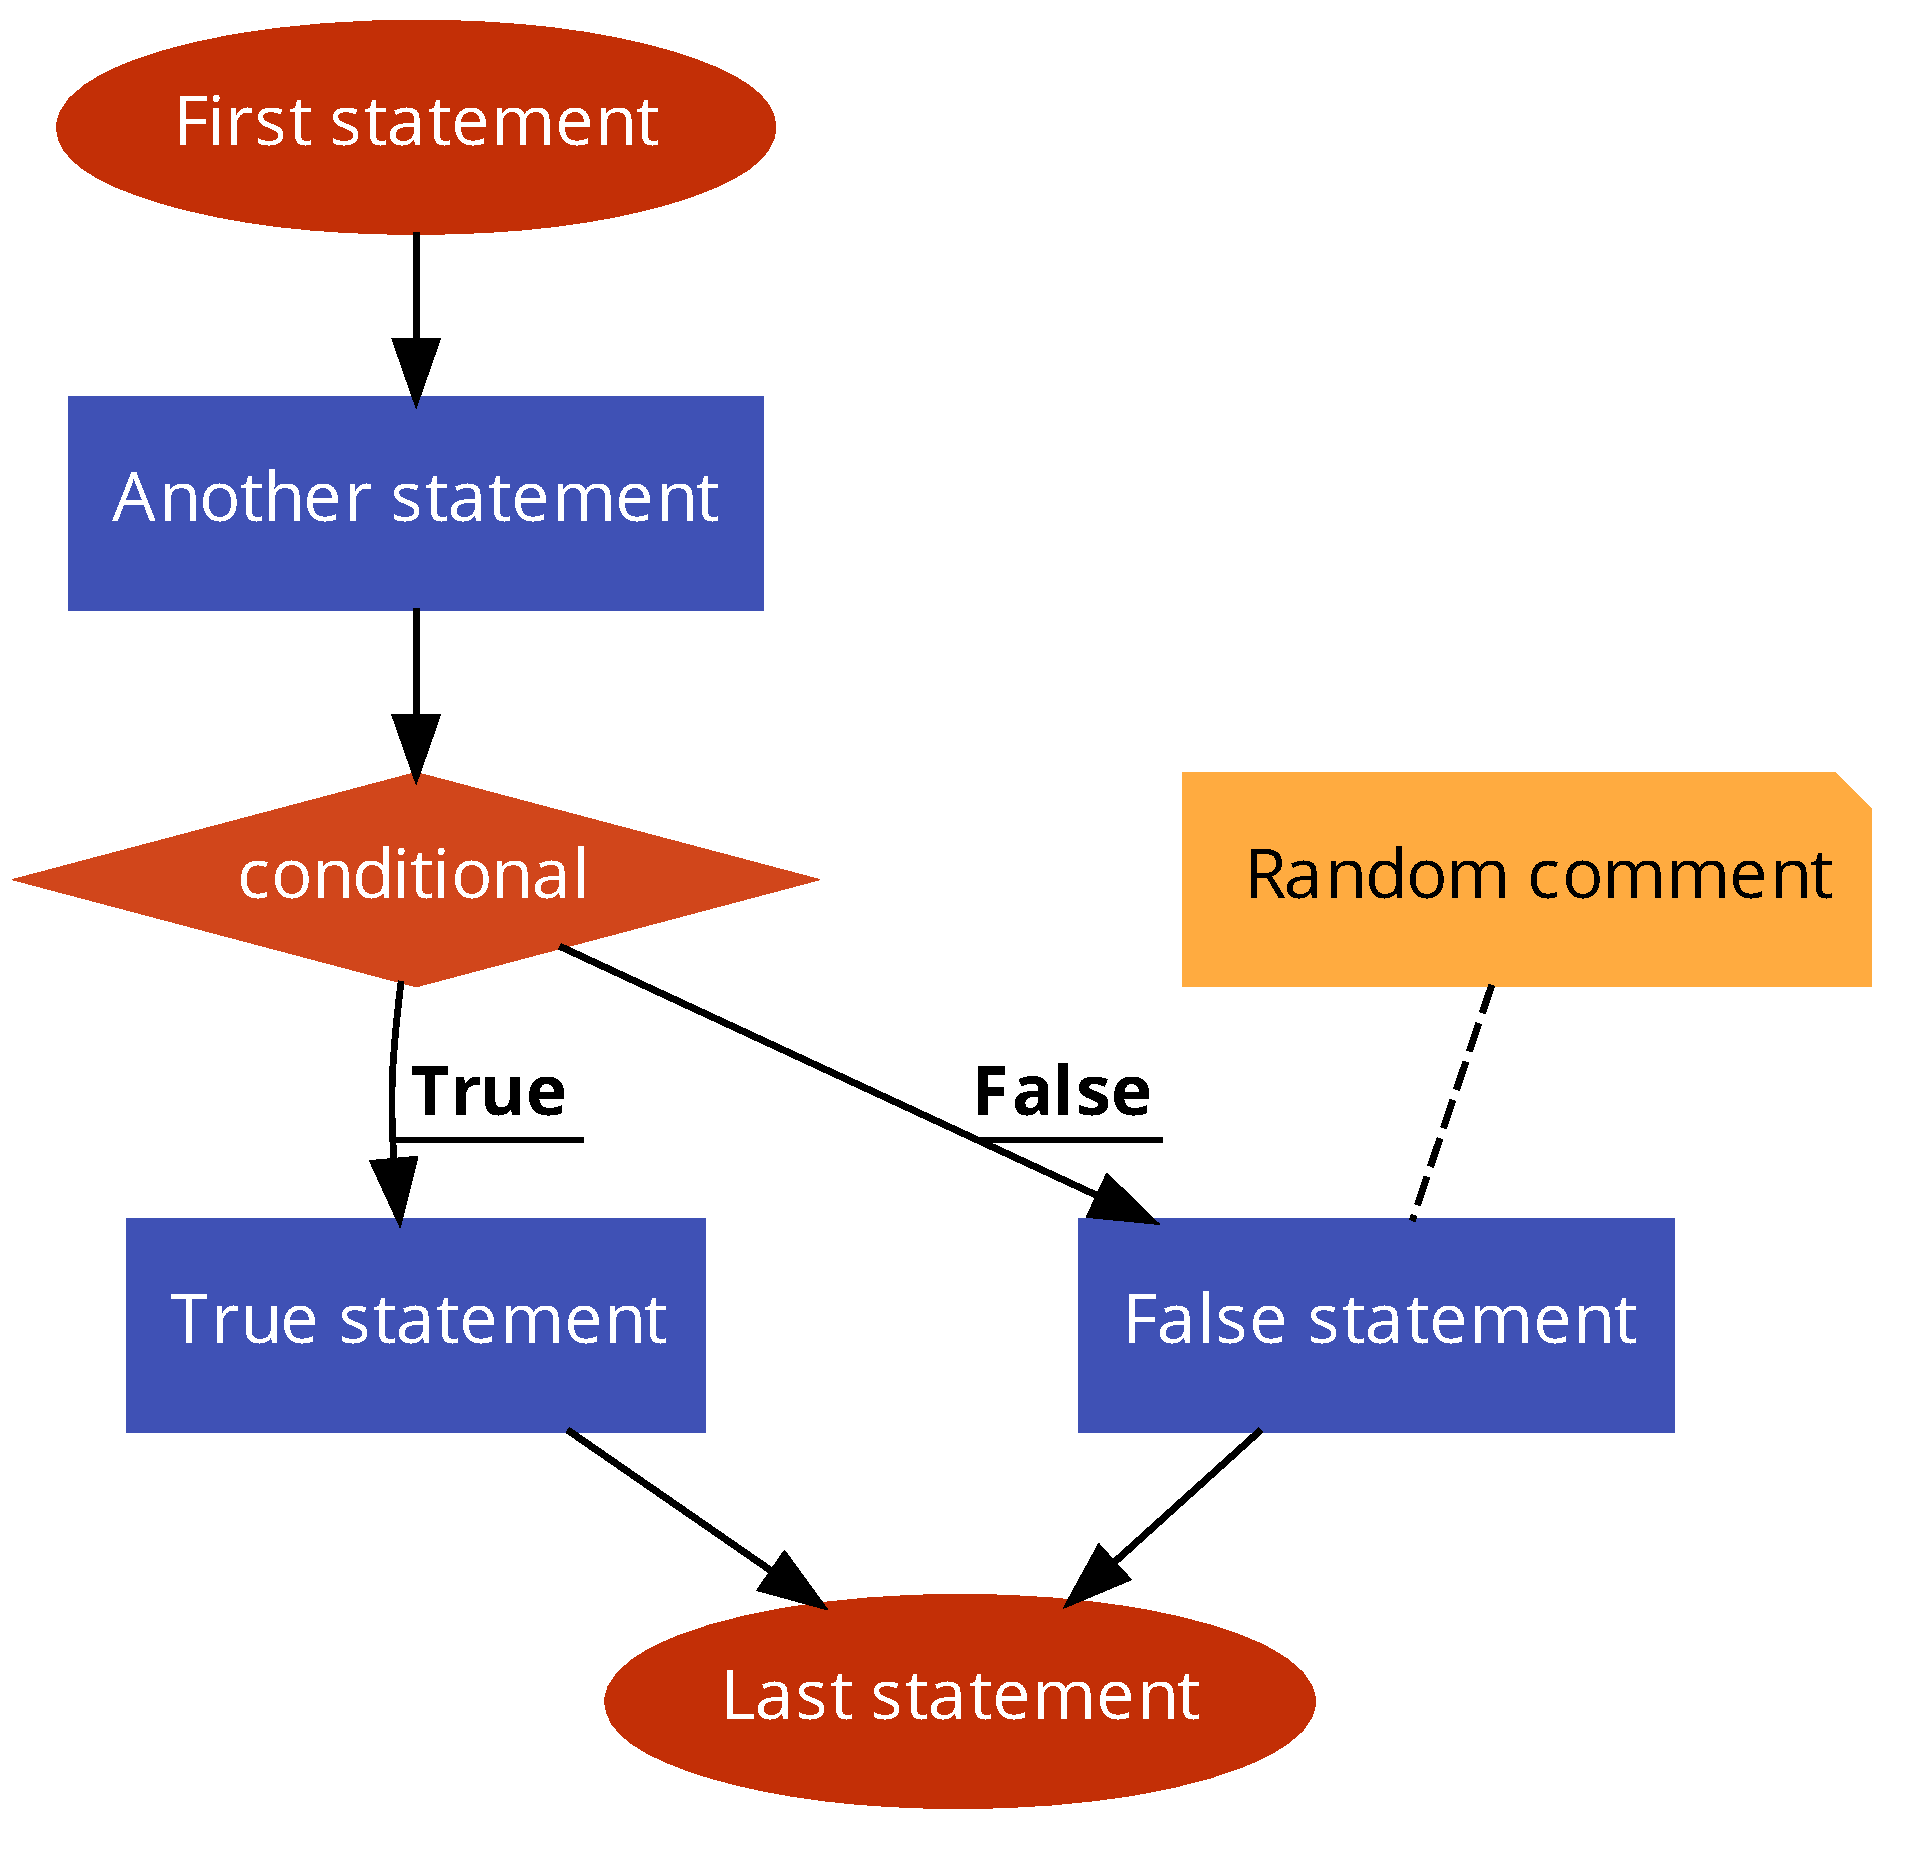
\includegraphics[scale=.28]{assets/chapter3/Code2FlowExample.pdf}
    \caption{The resulting flowchart from transpiling the Code2Flow code in \Cref{A Code2Flow program.}}
    \label{A Code2Flow flowchart.}
\end{figure}

If our C program inadvertently creates a ``correct'' flowchart, we can use a C compiler to test said program on the side. However, future changes to the C program are not guaranteed to successfully transpile to a new flowchart. \\

\textbf{Mermaid.js} is a DSL for rendering diagrams (including flowcharts) from a Markdown-inspired syntax. Even though we can construct many different diagrams with Mermaid.js, we will focus on the flowcharts. Like Code2Flow, they render flowcharts in real time. However, Mermaid.js \textit{will} warn us about syntax errors, and only re-render syntactically correct programs. \\

To construct a Mermaid.js flowchart, our source program must start with \texttt{flowchart TD}. Nodes can come in many different shapes, and are denoted by the types of brackets they use. For instance, \texttt{Node[ ]} displays a rectangle, \texttt{Node(( ))} displays a circle, and \texttt{Node\{ \}} displays a rhombus. Edges also come in many shapes: \texttt{$--$>} displays an arrow, \texttt{-.->} displays a dotted arrow, whilst \texttt{$---$} will display a simple link. \\

We can also add text to our nodes, by placing it within the brackets, like \texttt{Node[text]}. Arrows can also include text by breaking them up into two parts, like \texttt{$--$ text $--$>}.\footnote{The full documentation can be found here: \url{https://mermaid.js.org/syntax/flowchart.html}} \\

\begin{lstlisting}[caption={A mermaid.js program.}, captionpos=b, label={A mermaid.js program.}]
flowchart TD
    A([First statement])
        --> B[Another statement]
    B --> C{contidional}
    C -- True --> D[First statement]
    C -- False --> E[Second statement]
        %% Random comment
    D --> F([Last statement])
    E --> F
\end{lstlisting}

Just like with Code2Flow, the text inside these nodes can be anything. \Cref{A mermaid.js program.} shows a program written with Mermaid.js, and \Cref{A mermaid.js flowchart.} shows the corresponding flowchart. Contrary to Code2Flow, comments are ignored by the parser, and solely exist to aid the programmer. They must also be on their own lines. \\

\begin{figure}[ht]
    \centering
    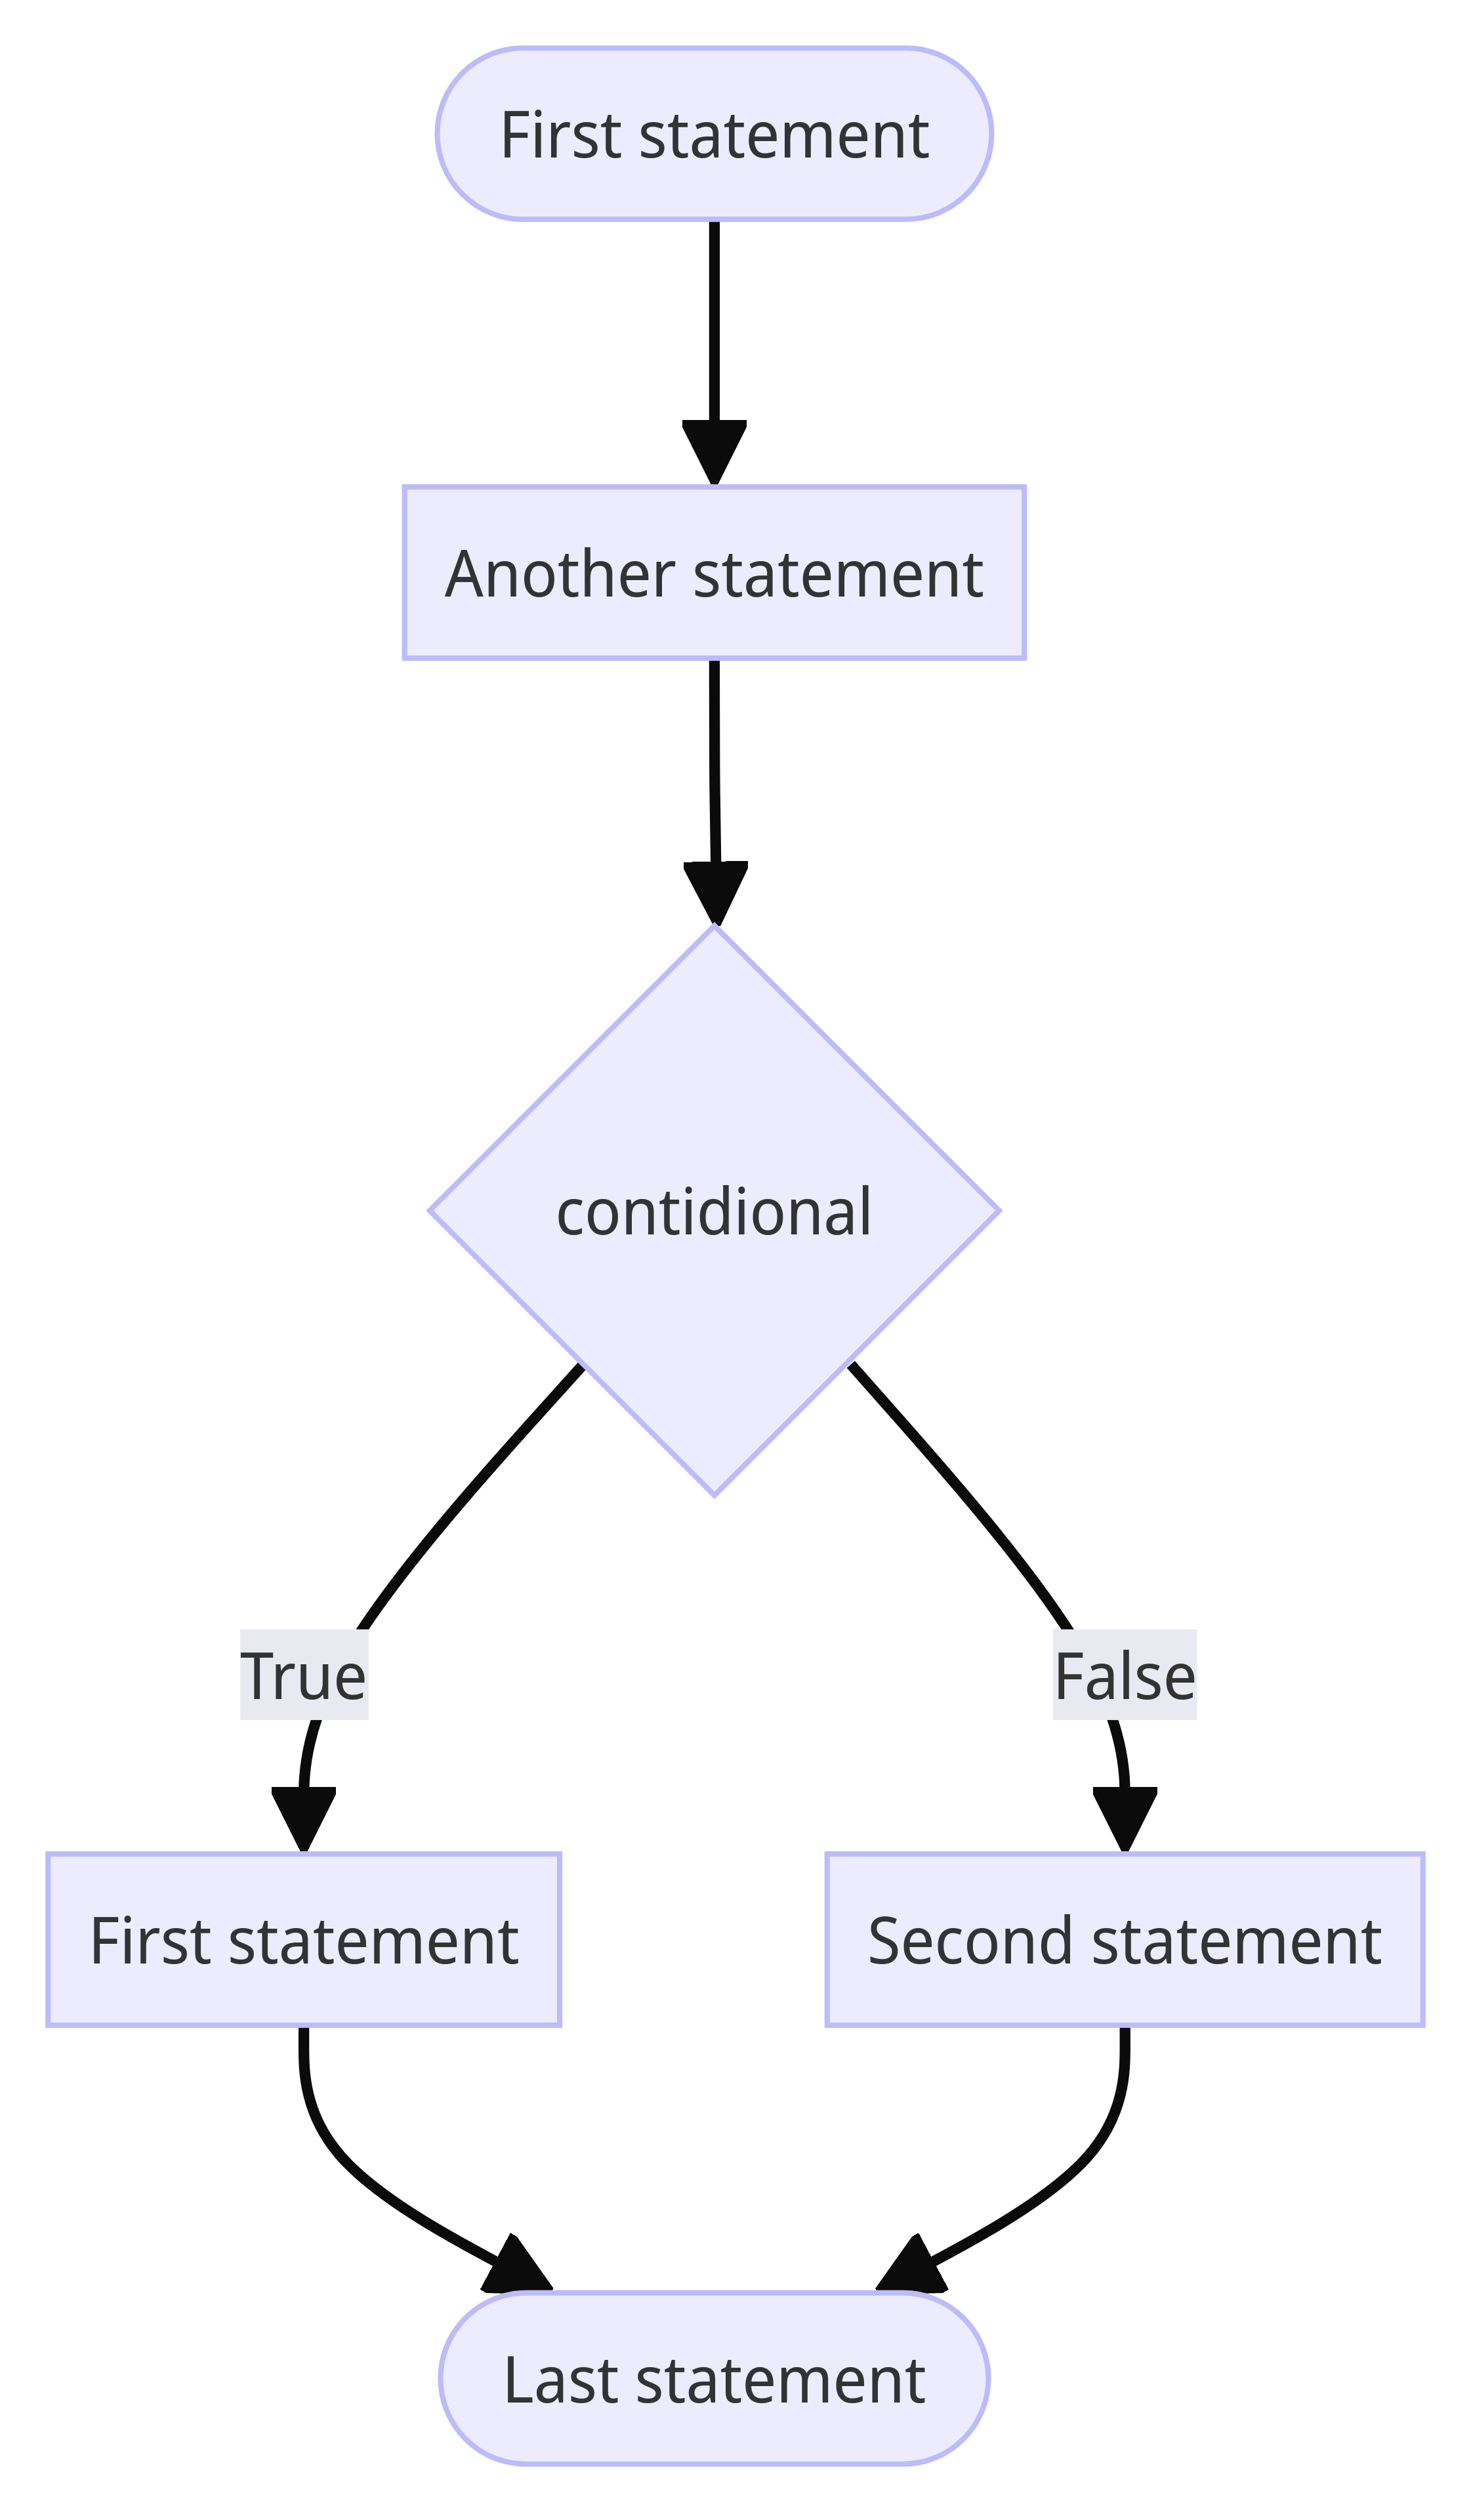
\includegraphics[scale=.07]{assets/chapter3/MermaidProgram.png}
    \caption{The resulting flowchart from transpiling the Mermaid.js code in \Cref{A mermaid.js program.}}
    \label{A mermaid.js flowchart.}
\end{figure}

The biggest drawback of Mermaid.js is that the syntax is very different from any programming language. This means pasting our source code will not yield any result, and we have to carefully translate our code every time. It also means that it is fully our responsability to maintain the abstraction level we want. Like Code2Flow, Mermaid.js has no way of letting us test our code.

\chapter{Design}

In this chapter, we introduce our tool Psnodig, and relevant design decisions. We also describe the design behind the Gourmet programming language, and the programs generating TBP and IBP.

\section{Proposed solution}

To solve the problem we are dealing with, we introduce Psnodig. We believe that Psnodig offers something unique in the context of this problem. Psnodig is a transpiler, intended to convert executable source programs to presentation-only target programs. \hfill \\

The programs discussed in Chapter 3 all do a very good job in their own right. The effort invested by developers, researchers and others involved is clearly reflected in both functionality and performance in each application. \hfill \\

However, none of them are particularly modifiable. We believe that a tool that combines these measures would be of even greater benefit. This way, the user does not have to operate with multiple tools at the same time. The user should also be able to add their own preferred output targets.

\forsup{``modifiable'' er ikke ordet jeg leter etter her. men kommer ikke på noe bedre akkurat nå..}

Additionally, these tools provide only the final result of conversion in the form of a PDF. We believe that the user would benefit from being able to modify the final result, in case the transition from the intermediate representation to the target is too lossy. \hfill \\

Where the programs primarily specialise in code generations, the DSLs are not executable. We believe that this is something that can be tremendously useful, and have therefore corporated an interpreter that works on the internal representation of Psnodig. To the best of our knowledge, a tool which combines all these methods does not currently exist. \hfill \\

Lastly, code generators traditionally do much more than directly translating data types to the target language. Therefore, we will refer to these programs simply as \textbf{writers} in the context of Psnodig, for the remainder of the thesis. \hfill \\

\forsup{Det er visstnok overraskende enkelt å skulle release Psnodig. Fikse noe cabal-greier og legge det ut på github, så skal man kunne kjøre `stack install`, og deretter skrive ting som `psnodig --tbp program.gt` istedenfor `stack run -- "--tbp" "program.gt"`!}

\section{Psnodig}

Psnodig is a collection of data types in Haskell, describing a computer program. As such, it does not provide a lot of functionality on its own. It is first when we add parsers and writers that it shows its usefulness. \hfill \\

Since we are free to add parsers and writers at will, only our imagination (and programming skills) can limit what we use it to convert. However, it is first and foremost intended as a tool for converting executable source programs to a presentation-only target programs. \hfill \\

To utilise Psnodig, source programs are parsed to an intermediate, internal representation. Later, this representation is used to convert the original program further into a new target program. This means that all source programs can be converted to the same target programs. \hfill \\

Psnodig also comes with an interpreter, which works on the internal representation. This means that we can add parsers and run the code, without having to write an additionaly interpreter or compiler. \hfill \\

The main benefit is that we can write our code once in a source language, test it, and when we are satisfied, transpile it to TBP and/or IBP thorugh the command line, rather than having to re-write it manually or search for a tool that can do that job for us. \hfill \\

\subsection{Syntax}

\forsup{blir egentlig syntax riktig ord å bruke her?}

The data types of Psnodig are presented in Listing ??. The entry point of a Psnodig program is \texttt{Program}, but since it consists of two lists and a \texttt{Maybe} data types, a minimal working example is actually an empty file. This flexibility allows our parsers and writers to utilise just as much, or as little, of the Psnodig syntax as we wish. \hfill \\

Most of the syntax will resemble the syntax of common programming languages. However, there are two statements that have been introduced specifically for Psnodig's real use case: Hash- and Annotation statements. \hfill \\

\begin{lstlisting}[caption={Psnodig's data types in Haskell}, captionpos=b, frame=trbl]
    data Program = Program [StructDecl] [Function]
                   (Maybe FunctionCall)

    data StructDecl = StructDecl String [Argument]

    data Struct = Struct String [Expression]

    data StructField = StructField Expression
                       Expression

    data Function = Function String [Argument]
                    [Statement]

    data FunctionCall = FunctionCall String
                        [Expression]

    data Argument = Argument String String

    data Statement =
          Assignment AssignmentTarget AssignmentValue
        | Loop Expression [Statement]
        | If Expression [Statement] (Maybe Else)
        | ForEach String Expression [Statement]
        | For String Expression Expression [Statement]
        | CallStmt FunctionCall
        | Return Expression
        | HashStmt Statement
        | AnnotationStmt String [Statement]
        | Break
        | Continue

    data AssignmentTarget =
          VariableTarget String
        | ListIndexTarget String [Expression]
        | StructFieldTarget StructField

    data AssignmentValue =
          ExpressionValue Expression
        | StructValue Struct

    data Else =
          ElseIf Expression [Statement] (Maybe Else)
        | Else [Statement]

    data Expression =
          Constant Value
        | VariableExp String
        | BinaryExp Operator Expression Expression
        | ListIndex String [Expression]
        | CallExp FunctionCall
        | Not Expression
        | StructExpr Struct
        | StructFieldExp StructField

    data Operator =
          Plus
        | Minus
        | Times
        | Division
        | LessThan
        | LessThanEqual
        | GreaterThan
        | GreaterThanEqual
        | Equal
        | NotEqual
        | And
        | Or
        | Modulo

    data Value =
          Nil
        | Boolean Bool
        | Number Integer
        | Text String
        | List [Expression]
        | HashSet (Set.Set Expression)
        | HashMap (Map.Map Expression Expression)
        | StructVal [(String, Value)]
\end{lstlisting}

Hash statements are statements intended to be parsed by the interpreter, but ignored by the writers. This lets us abstract away things that should be obvious to our audience, or perhaps things that have already been stated elsewhere, but still need to be stated for our programs to actually run. The name derives from how we can write single line comments in Python with a hash symbol. \hfill \\

A common use case of this is when a lower case \texttt{n} is often used to denote amounts in TBP. By using a hash statement, we avoid including superflous function calls to length-functions when it is obvious what \texttt{n} symbolises. \hfill \\

Annotation statements are statements that allow us to add an extra layer of abstraction to our output targets. The first string is what is presented, in natural language, whilst the list of statements is read by the interpreter. \hfill \\

A common use case of this is when we wish to swap two elements in a list. In many programming languages, when swapping two elements \texttt{a} and \texttt{b}, we have to assign \texttt{a} to a temporary variable, before assigning \texttt{a} to \texttt{b}, and finally assigning \texttt{b} to that temporary variable. These three implementation-specific lines could easily be abstracted with \texttt{swap a and b}. \hfill \\

These two statements are particularly useful when a piece of code is not crucial to the program's logic, or when the code is very implementation specific. The statement list can also be empty, which lets us explain things solely with natural language when deemed necessary. \hfill \\

\subsection{Interpreter}

A big selling point of Psnodig, is that in addition to being a transpiler, it also comes with an interpreter, which works on the AST. For a program to be transpiled, it only needs to be syntactically correct. However, this does not guarantee that the program works as the user intended. Thus, Psnodig provides users with the ability to test their programs before they are transpiled and later presented, which in many cases can be crucial. \hfill \\

Take the program presented in Listing ?? as an example. The function \\ \texttt{printEvenNumbers} takes two arguments: a list of numbers and the list's length. Then we iterate through this range, and proceed to print every number in the list that is even. However, we check for evenness by doing \texttt{if i \% 2 == 0}, but really we intend to do \texttt{if numbers[i] \% 2 == 0}. The difference is subtle, but by running the program we quickly realise the error when the screen displays 47, 79 and 93 rather than 46 and 22. \hfill \\

\begin{lstlisting}[caption={A syntactically correct program with a subtle logical error}, captionpos=b, frame=tlrb]{Name}
func printEvenNumbers(numbers list, length int) {
    for i := 0, length-1 {
        if i % 2 == 0 {
            print(numbers[i])
        }
    }

    return 1
}

printEvenNumbers([47, 46, 79, 22, 93], 5)
\end{lstlisting}

As seen from the grammar in Listing 4.1, programs consist of three parts: A list of struct declarations (which can be empty), a list of function declarations (which can also be empty), and lastly, an optional function call. The function call works as the entry point of the interpreter.

\subsubsection{Scope}

Psnodig works with both a global and a local scope. All structs and functions are global, and can be accessed from any other functions. For instance, functions can be mutually recursive. Variables, on the other hand, are always local, and a variable declared in function \texttt{f} cannot be accessed in function \texttt{g}, unless passed as an argument. \\

Listing ?? shows two syntactically valid programs, but Listing ?? (a) will yield an error, whilst Listing ?? (b) will eventually return 1. \\

\begin{minipage}{.45\textwidth}
\begin{lstlisting}[caption=Code with error, captionpos=b, frame=tlrb]{Name}
func f() {
    n := 5
    return g()
}

func g() {
    return n
}

f()
\end{lstlisting}
\end{minipage}\hfill
\begin{minipage}{.45\textwidth}
\begin{lstlisting}[caption=Code without error, captionpos=b, frame=tlrb]{Name}
func f() {
    n := 5
    return g(n)
}

func g(n int) {
    return n
}

f()
\end{lstlisting}
\end{minipage}

Psnodig supports nested scopes as indicated in the \texttt{For String Expression Expression [Statement]} structure within the \texttt{Statement} data type. The two \texttt{Expression} data types define a range, whilst the \texttt{String} data type serves as an identifier that binds to all numbers within this specified range (inclusive). \\

The statements are then executed repeatedly for each value in this range, with the identifier reflecting the current value on each iteration. Once the loop terminates, the identifier is automatically unbound, and no longer exists in the context.

\subsubsection{Peculiarities}

As seen, Psnodig prohibits two types of for loops. \texttt{For String Expression [Statement]} is discused in the previous subsection, but we also have \texttt{ForEach String Expression [Statement]}.

\forsup{Jeg vil egentlig endre dette til å være ForEach String Iterable [Statement], også begrenser vi Iterable til Variabler og ListIndex}

\subsubsection{Standard Library}

The interpreter provides several built-in functions, which are also found in most programming languages. They are also reflected in the TBP writer. If the function call fails, due to e.g. wrong number of arguments or arguments having the wrong type, the program will stop and the user will receive an explanatory error message. \\

\textbf{print($x_{1}$, $..$, $x_{n}$)}, which takes $n \in \mathbb{N}$ arguments. The arguments must be of type \texttt{Expression}, and each argument is printed on their own line in terminal. The function returns the number of arguments passed to it. \\

\textbf{length($x$)}, which takes one argument. The argument must be either a \texttt{Text}, \texttt{List}, \texttt{HashSet}, or \texttt{HashMap}. The function returns the length of its argument: Number of characters in text, number of elements in list and hashset, and number of mappings in hashmap. \\

\textbf{ceil($n$)} and \textbf{floor($n$)}, which take one number $n \in \mathbb{Q}$ as argument. The return value will be rounded up or down to the nearest $n' \in \mathbb{N}$, respectively. \\

\textbf{min($n_{1}$, $..$, $n_{n}$)} and \textbf{max($n_{1}$, $..$, $n_{n}$)}, which takes $m \in \mathbb{N}$ arguments. The arguments themselves must also be an $n \in \mathbb{N}$. The return value will be the smallest value and the largest value, respectively, amongst the arguments. \\

\textbf{append($x$, $xs$)}, which takes two arguments. The first argument must be an \texttt{Expression}, and the second argument must be a \texttt{List}. The function will append \texttt{x} to the end of \texttt{xs}, thus modifying the list. The function returns the number 1 if everything went well. \\

\textbf{add($x$, $hs$)} and \textbf{add($k$, $v$, $hm$)}, which is an overloaded function, taking either two or three arguments. In the first case, it adds an \texttt{Expression} $x$ to a \texttt{HashSet} $hs$. In the other case it maps an \texttt{Expression} $k$ to an \texttt{Expression} $v$ in a \texttt{HashSet} $hm$. The function always returns 1 upon success. \\

\textbf{get($k$, $hm$)}, which takes two arguments, an \texttt{Expression} $k$ and a \texttt{HashMap} $hm$. If $k$ is a key in $hm$, the function will return the value that $k$ maps to in $hm$. \\

\textbf{in($x$, $xs$)}, which takes two arguments, an \texttt{Expression} $x$ and either a \texttt{List}, \texttt{HashSet}, or \texttt{HashMap}. The function will check if $x$ exists in $xs$, and return $True$ or $False$ accordingly.

\subsection{Testing}

Psnodig is not accompanied by any testing framework, but we have done some testing with QuickCheck \hfill \\

\forsup{Har ingen tester akkurat nå. Prøvde å teste 'AST -> Gourmet -> AST' tidligere, men la det på is. Kan det være en fin ting å teste?}

\forsup{en annen ting som kan være interessant å teste: programmer som transpiler til latex, uten å krasje. opplever noen ganger at jeg har glemt en edge case eller noe, eller til og med glemt å importere et bibliotek. vet ikke helt hvordan denne testen skulle sett ut, men det gir jo grunnlag for å si at det er ``trygt'' å bruke psnodig, og at det er ``komplett'' i konteksten av seg selv}

\section{Gourmet}

To make sure Psnodig works at all, we depend on having at least one input target and one output target. When it comes to input language, we have two plausible alternatives: Use an existing programming language, or design a new one. We decided to opt for the latter. \hfill \\

In the context of Psnodig, we just need to build a parser that can translate programs in the source language to the intermediate representation. There are several reasons as to why designing a new language for the purpose of proof of concept is a good choice. \hfill \\

For one, it demonstrates the general effort to add an entirely new input target for Psnodig. This can motivate others to add their own. Because the  \hfill \\

Another reason is that selecting a single programming language to encompass all needs is not feasible. For instance, the largest university in southern Norway uses Python for its introductory programming course\footnote{Course page for \textit{Introduction to object-oriented programming} at the University of Oslo:~\url{www.uio.no/studier/emner/matnat/ifi/IN1000/}}, whilst the largest university in northern Norway prefers C\footnote{Curriculum for \textit{Introduction to programming and the computer's mode of operation} at the University of Tromsø:~\url{www.bibsys-c.alma.exlibrisgroup.com/leganto/readinglist/lists/10569365600002205?institute=47BIBSYS_UBTO&auth=SAML}}. The largest university in Greece opts for Java~\footnote{Course page for \textit{Introduction to Computer Science} at the University of Athens:~\url{www.dept.aueb.gr/en/dmst/content/introduction-computer-science}}, and Harvard's renowned CS50 course introduces students to both JavaScript and SQL\footnote{Course page for \textit{Introduction to Computer Science} at the University of Harvard:~\url{www.pll.harvard.edu/course/cs50-introduction-computer-science}}. \hfill \\

\forsup{Lars kommenterte en gang at en fotnote burde ligge på utsiden høyresiden av punktum. Gjelder det også over her? er det bedre med feks ``tekst her og tekst der.1 2'' istedenfor ``tekst her 1 og tekst der 2.''? hvis det ga mening}

What the languages of introductory courses to computer science do have in common, is that they tend to be within the imperative paradigm of computer programming. As such, we did not want to stray too far away from that, and have allowed ourselves to mainly be inspired by the Go programming language. The language started out as a pure subset of Go, hence its name: A gourmet portion of Go.

\subsection{Lexical Aspects}

\subsubsection{Identifiers and keywords}

An identifier in Gourmet is used to reference either a struct, function or variable. Identifiers are also restricted to begin with a letter, followed by an arbitrary number of letters, numbers, and single quotes. \textbf{variable}, \textbf{var1able’} and \textbf{g0urmetVar1able''’'} are all valid Gourmet identifiers, whilst \textbf{1variable} and \textbf{'variable} are both not. Additionally, an identifier can not shadow keywords. \hfill \\

In total, there are 40 keywords in Gourmet, with 14 of them sharing structures with identifiers. They are \textbf{while}, \textbf{if}, \textbf{func}, \textbf{true}, \textbf{false}, \textbf{return}, \textbf{else}, \textbf{for}, \textbf{break}, \textbf{continue}, \textbf{struct}, \textbf{not}, \textbf{map} and \textbf{set}. These keywords are also reserved, which means that we cannot define an identifier \textbf{while} or \textbf{func}. The remaining keywords will be presented in Section ?? \hfill \\

We can define functions which clashes with library functions in Psnodig, but when trying to run that program, we receive an error message when our program tries to call those functions. This will happen even if we overload our functions with a different number of arguments, thus in reality removing the ambiguity. That means that we cannot run our own \textbf{print} function. However, we can always define a function e.g. \textbf{print’} or \textbf{print1}. \hfill \\

\subsubsection{Comments}

As there are no data types for comments in Psnodig, they must be handled entirely by Gourmet. The language supports both single- and multi-line comments, both identical to the ones found in most C-like languages like C itself, Java, Go and more. \hfill \\

Single-line comments begin with a double forward slash \textbf{//}, and extends to the end of that line. Multi-line comments start with a forward slash and a star \textbf{/*}, and end with a star and a forward slash \textbf{*/}. Multi-line comments cannot be nested, which means that the first \textbf{*/} after a \textbf{/*} will end that comment, no matter how many \textbf{\*} preceeds it. \hfill \\

\subsubsection{Whitespace}

Whitespace can be defined as spaces, newlines and tabs. Gourmet does not differentiate between either of them, and we can use them in our programs exactly how we wish. \hfill \\

Listing 4.1, Listing 4.2 and Listing 4.3 show a semantically identical program. We define a function \textbf{f} which again defines \textbf{a} to be a list with two elements, before returning it. Lastly, the fuction is called. All three programs will be successfully parsed, and have the same internal representation in Psnodig. \hfill \\

\begin{lstlisting}[caption={f with a standard amount of whitespace}, captionpos=b, frame=tlrb]
    func f() {
        a := [1, 2]
        return a
    }

    f()    
\end{lstlisting}

\begin{lstlisting}[caption={f with a lot of whitespace}, captionpos=b, frame=tlrb]
    func f()
    {
        a       :=
            [1   ,   2]
        return
        a
    }
    
    f   (   )
\end{lstlisting}

\begin{lstlisting}[caption={f with no whitespace}, captionpos=b, frame=tlrb]
    funcf(){a:=[1,2]returna}f()
\end{lstlisting}

\forsup{har tatt mye inspirasjon herfra: \url{https://github.uio.no/compilerconstruction-inf5110/compila/blob/master/doc/languagespec/compila.pdf} uten å kildeføre noe. her er jeg veldig usikker på hva jeg skal gjøre! har jeg kopiert for mye? KAN jeg i det hele tatt kildeføre noe slikt?}

\subsection{Types}

Gourmet is dynamically typed, which means that we do not have to specify the type of variables and return type of functions. In fact, Gourmet does not even \textit{allow} it. When defining structs and function arguments, however, we have to provide type hints on the form \textbf{name \textit{type}}. \hfill \\

The reason behind this choice is solely to improve code readability. When defining a variable, the value will always be present on the right hand side. When working with function arguments, however, we can never be entirely sure what a user decides to pass. With type hints, their ``intended use'' instantly becomes clear. \hfill \\

There are, however, four base types that all values will have: \textbf{Boolean}, \textbf{Number} and \textbf{Text}, and \textbf{nil}. A boolean is either true or false, a number is an arbitrarily large number, and a text is an arbitrarily combination of letters within a pair of double quotes. Nil indicates the absence of a value, and is mostly assigned as a placeholder. \hfill \\

Essentially, types associate data values into classes and provide rules for how these classes should interact[kilde]. Sometimes - to solve specific problems - the base types Gourmet offers might not suffice. Therefore, we can create our own types through structs. Structs in Gourmet work exactly the same way they do in languages like C and Go, containing instance variables, but no methods or constructors, like in languages like Python and Java. \hfill \\

Listing 4.4 shows how we can create a struct for modelling a tree data structure, and Listing 4.5 shows how they can be initialised. \hfill \\

\begin{lstlisting}[caption={A Gourmet struct Tree, with instance variables value, left and right}, captionpos=b, frame=tlrb]
    struct Tree {
        value int,
        left Tree,
        right Tree
    }
\end{lstlisting}

\begin{lstlisting}[caption=A function to initialise three tree structs and return the last one,captionpos=b, frame=tlrb]{Program}
    func f() {
        tree := struct Tree(10, nil, nil)
        tree' := struct Tree(20, nil, nil)
        tree'' := struct Tree(15, tree, tree')
        return tree''
    }
\end{lstlisting}

\subsection{Syntax}

\subsubsection{Grammar}

Gourmet's EBNF grammar is presented in Figure ??. EBNF (short for Extended Backus-Naur form) is a notation for expressing a programming language's grammar. It is an extension of BNF (short for Backus-Naur form) that was developed in the 1960s to describe the syntax of the ALGOL programming language [kilde]. We could have used the original BNF notation, but EBNF allows us to present it more succinctly. \hfill \\

In this variant of EBNF, we use the following meta symbols:

\begin{lstlisting}
    -> { } [ ] " ( ) |
\end{lstlisting}

Arrows indicate the application of a rule. Curly brackets indicate repetition of 0 or more times (much like the reflexive arrow in Figure 2.1). Square brackets indicate binary presentness. Vertical bars indicate option. Anything wrapped in double quotes is a keyword. \hfill \\

Non-terminals are written in upper case. There are also four terms written in upper case, that do not have production rules: \textbf{NAME}, \textbf{TEXT}, \textbf{NUMBER}, \textbf{STRING\_LITERAL}. NAME is an identifier, already described in Section 4.3.1.1. TEXT is any combination of UFT-8 symbols. It is only present once, and is intended for ``hiding'' code under an abstracting layer of natural language. NUMBER is any combination of whole numbers. STRING\_LITERAL is similar to TEXT, but additionally it is wrapped in double quotes. \hfill \\

\forsup{Bør jeg forklare dette mer? F.eks. dette med terminals og non-terminals osv.}

\begin{figure}
    \begin{subfigure}[ht]{1\linewidth}
        \begin{tabular}{c}
            \begin{lstlisting}
PROGRAM          -> { STRUCTDECL } { FUNCTIONDECL }
                    [ FUNCTIONCALL ]

STRUCTDECL       -> "struct" NAME "{" { ARGUMENT } "}"

FUNCTION         -> "func" NAME "(" [ ARGUMENT { ","
                    ARGUMENT } ] ")" "{" { STATEMENT }
                    "}"
ARGUMENT         -> NAME NAME

STATEMENT        -> ASSIGNMENT | LOOP | IF | FOREACH
                    | FOR | FUNCTIONCALL | ANNOTATIONSTMT
                    | # STATEMENT | "return" EXPRESSION
                    | "break" | "continue"

ASSIGNMENT       -> ASSIGNMENTTARGET ":=" ASSIGNMENTVALUE

LOOP             -> "while" EXPRESSION "{" { STATEMENT } "}"

IF               -> "if" EXPRESSION "{" { STATEMENT } "}"
                    [ ELSE ]

FOREACH          -> "for" NAME ":=" EXPRESSION "{"
                    { STATEMENT } "}"

FOR              -> "for" NAME ":=" EXPRESSION ","
                    EXPRESSION "{" { STATEMENT } "}"

FUNCTIONCALL     -> NAME "(" EXPLIST ")"

ANNOTATIONSTMT   -> "@" "{" TEXT "}" "{" { STATEMENT } "}"

ASSIGNMENTTARGET -> NAME | LISTINDEX | STRUCTFIELD

ASSIGNMENTVALUE  -> EXPRESSION | STRUCT

ELSE             -> "else" IF | "else" "{" { STATEMENT } "}"

EXPRESSION       -> VALUE | NAME | LISTINDEX
                    | EXPRESSION OPERATOR EXPRESSION
                    | FUNCTIONCALL | "not" EXPRESSION
                    | STRUCT | STRUCTFIELD

LISTINDEX        -> NAME "[" EXPRESSION "]" { "["
                    EXPRESSION "]" }

OPERATOR         -> "+" | "-" | "*" | "/" | "<" | "<="
                    | ">" | ">=" | "==" | "!=" | "&&"
                    | "||" | "%"

            \end{lstlisting}
        \end{tabular}
    \end{subfigure}
    \label{fig:gourmet-grammer1}
\end{figure}

\begin{figure}
    \begin{subfigure}[ht]{1\linewidth}
        \begin{tabular}{c}
            \begin{lstlisting}
STRUCT           -> NAME "(" EXPLIST ")"

STRUCTFIELD      -> EXPRESSION "." EXPRESSION

VALUE            -> "nil" | "true" | "false" | NUMBER
                    | STRING_LITERAL | "[" EXPLIST "]"
                    | "map" "{" [ PAIR { "," PAIR } ] "}"
                    | "set" "{" EXPLIST "}"

PAIR             -> EXPRESSION ":" EXPRESSION

EXPLIST          -> [ EXPRESSION { "," EXPRESSION } ]

            \end{lstlisting}
        \end{tabular}
    \end{subfigure}
    \setcounter{figure}{1}
    \caption{The EBNF grammar of the Gourmet programming language}
    \label{fig:gourmet-grammer1}
\end{figure}

\subsubsection{Precedence and Associativity}

The precedence of Gourmet operators is ranked in the following order, from highest to lowest:

\begin{enumerate}
    \item $*$ and $/$ and $\%$
    \item $+$ and $-$
    \item $<$, $<=$, $>$ and $>=$
    \item $==$ and $!=$
    \item $\&\&$ and $||$
    \item $.$ (to access fields of a struct)
    \item not
\end{enumerate}

This means that if we wish to calculate the sum of the tree values from Listing 4.5, we cannot write \texttt{tree.value + tree'.value + tree''.value}, because the parser will parse \texttt{(p.(value + p').(value + p'')).value}. Therefore, we have to include parentheses explicitly: \texttt{(tree.value) + (tree'.value) + (tree''.value)}. \hfill \\

All binary operations are left-associative.

\section{TBP Writer}

Our TBP writer takes an internal representation of Psnodig and produces a LaTeX file. As previously stated, we are not attempting to create a ground truth for pseudocode. Therefore, we have chosen to produce the pseudocode with the Algorithm2e package. \hfill \\

\forsup{Akkurat nå håndterer vi ikke Input, Output og Caption. Hvordan dette gjøres er nok ikke så farlig. Må bestemme om dette skal bakes inn i Psnodig, eller om vi f.eks. skal hente det fra kommandolinjen idet noen kjører ``stack run -- tbp program.gt''}

Structs and the initial function call are not converted to pseudocode. For one, we believe that function calls are rarely cruical to the algorithm itself, and structs will always be implementation specific. \hfill \\

\forsup{jeg sverger jeg hadde en til grunn}

\subsection{Algorithm2e}

\forsup{Bør jeg skrive en eller annen intro om pakken?}

Algorithm2e allows us to define our own keywords with the \texttt{\textbackslash SetKw\{\}\{\}} command. These are macros, where if we define \texttt{\textbackslash SetKw\{KwBreak\}\{break\}}, we can write \texttt{\textbackslash KwBreak}, and \texttt{break} will be printed. \hfill \\

There are also more specific macros, like \texttt{\textbackslash SetKwProg\{proc\}\{Procedure\}\{is\}\{end\}}. This is used to initialise programs, and denotes a special syntax for the program. Listing ?? (a) shows an example program, and Listing ?? (b) shows the subsequent compiled result. For our TBP writer, we decide to ignore the last two parameters, because we do not believe they add enough value to the final result. \hfill \\

\forsup{fiks eksempel til den over.}

Another special macro is \texttt{\textbackslash SetKwFunction\{f\}\{f\}}. This allows us to write e.g. \texttt{\textbackslash f\{arg1, arg2, arg3\}}, which looks like displays \f{arg1, arg2, arg3}. \hfill \\

Since we are still in a LaTeX environment, and backslashes are used for macros in standard LaTeX too, we have to be careful. We are not allowed to rename internal macros. For instance, \texttt{\textbackslash m} is already a macro in LaTeX, thus attempting to compile a file with \texttt{\textbackslash SetKwFunction\{m\}\{m\}} will lead to multiple errors and ruin the final output.

\subsection{Compatibility with Psnodig}

As previously mentioned in Section ??, all Psnodig library functions taken into consideration by our TBP writer. The function call \texttt{length(list)} is transpiled with the cardinality symbols to $\abs{list}$. The function call \texttt{append(x, xs)} is transpiled with natural language, to \texttt{append x to xs}, to avoid ambiguity. \\

Mathematical expressions are also taken into consideration. For instance, the Expression \texttt{BinaryExp Division (Constant (Number 2)) (Constant (Number 1))} will show $\frac{2}{1}$, rather than \texttt{2/1}. Similarly, an expression with multiplication will be displayed as \texttt{n $\cdot$ n} rather than \texttt{n * n}. \\

To work with mathematical symbols in LaTeX we use the packages \textbf{amsmath} and \textbf{commath}. \\

We also declare some macros to match the syntax of Psnodig. For instance, all programs come with \texttt{\textbackslash SetKw\{Return\}\{Return\}} and \texttt{\textbackslash SetKw\{False\}\{false\}}. Code like \texttt{return 5} or \texttt{v := false} will be presented with the keywords in boldface. \\

\forsup{Before a program is transpiled to TBP, another program is ran to see which keywords are used, and only these are imported in the resulting LaTeX file. So, unless the program actually contains a \texttt{Return} expression, the macro will not be included. This makes the program less bloated, and easier to navigate if the user wishes to modify something themselves.}

\subsection{Output}

Transpiling a program to TBP yields two files: a corresponding LaTeX file, and a PDF version of said LaTeX file. \\

Because the LaTeX file is built from Psnodig's internal representation, and not directly from the source program, formatting is not taken into account. This means that a program like

\texttt{ func f()\{v:=5 returnv\}f() } \\

will not be transpiled to \\

\texttt{ \textbackslash proc\{\$\textbackslash f()\$\}\{\$\textbackslash texttt\{v\}\textbackslash gets5\$\textbackslash ; \textbackslash Return\$v\$\textbackslash;\} } \\

but instead

\begin{verbatim}
    \proc{$\f()$}{
        $\texttt{v} \gets 5$ \;
        \Return $v$ \;
    }
\end{verbatim}

even though they would produce the same PDF. The LaTeX files also include \texttt{ \textbackslash SetKwProg\{proc\}\{Procedure\}\{\}\{\} } and \texttt{ \textbackslash SetKwFunction\{f\}\{f\} }. We include the \texttt{linesnumbered}- and \texttt{ruled} parameters from algorithm2e, purely for aesthetic reasons. Listing ?? (a) shows the program we just mentioned with these parameters, whilst Listing ?? (b) shows the same program without the parameters. \\

\begin{figure}[ht]
\centering
\begin{subfigure}{.5\textwidth}
  \centering
  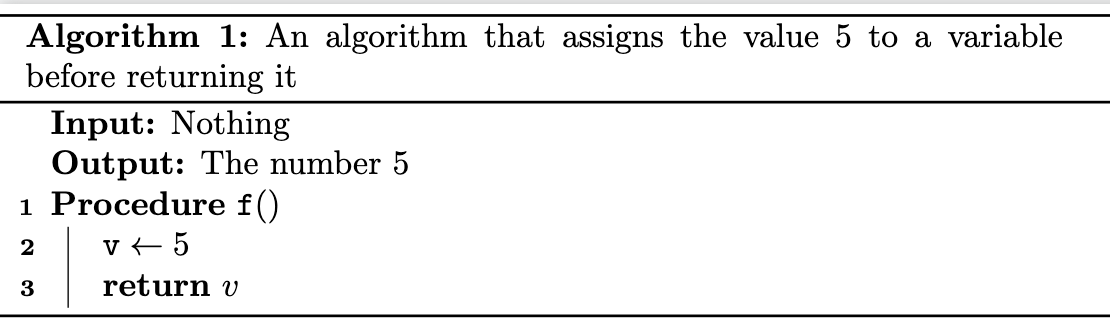
\includegraphics[width=.9\linewidth]{assets/return5pretty.png}
  \caption{f with extra parameters}
  \label{fig:sub1}
\end{subfigure}%
\begin{subfigure}{.5\textwidth}
  \centering
  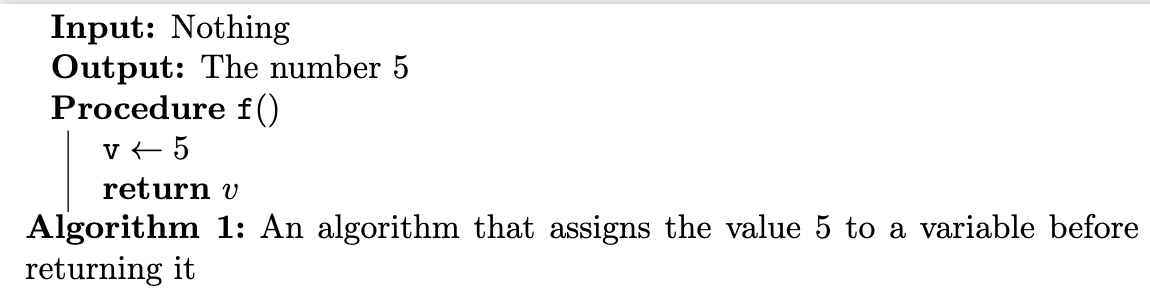
\includegraphics[width=.9\linewidth]{assets/return5ugly.png}
  \caption{f without extra parameters}
  \label{fig:sub2}
\end{subfigure}
\caption{TBP of an algorithm f, with and without extra visual parameters}
\label{fig:test}
\end{figure}

\forsup{If, for some reason, we do not want a PDF to accompany our LaTeX file, we can put an extra flag when calling the program. The flag is ``--nopdf'', and the whole command would be ``psnodig --tbp --nopdf program.gt''.}

\forsup{Burde jeg skrive noe om flagg og sånt i Design av Psnodig?}


\section{IBP Writer}

Our IBP writer works much like the TBP writer: An internal representation of Psnodig is transpiled to a LaTeX file. The flowcharts are created with the TikZ package. \\

Just like the TBP writer, our IBP writer only transpiles the topmost function, ignoring structs and the initial function call. Our reasoning is the same as earlier. To transpile a program to IBP, we run \texttt{psnodig --ibp <program>} in the command line.

\subsection{TikZ}

TikZ is a massive package. We actually used TikZ to create the FSA example in Section 2.1.2. \\

\forsup{Bør jeg skrive en eller annen intro om pakken?}

Our flowcharts mainly consist of three macros: \texttt{\textbackslash tikzstyle}, \texttt{\textbackslash node}, and \texttt{\textbackslash edge}. \texttt{tikzstyle} lets us choose what our nodes look like, \texttt{ndode} lets us draw the nodes we want, and \texttt{edge} lets us add an edge between nodes. \\

Each node in our flowcharts represents a statement, except the top one, which is the function name. The visual design is simple: the top node and all nodes of return statements are dark rectangles with rounded edges. Decision nodes, where the program diverges, are yellow diamonds. These are while-, for- and if-statements. The remaining statements are purple rectangles. The edges are thin arrows. \\

Tikzstyles are written on the form

\begin{verbatim}
    \tikzstyle {style name} =
        [ shape
        , minimum width = x cm
        , minimum height = y cm
        , text <position>
        , draw = colour
        , text = colour'
        , fill = colour''
        ]
\end{verbatim}

The style name will be referenced later by nodes. The shape can be a rectangle, circle or coordinate, but we can import more libraries to get shapes like e.g. diamonds. The three colours refer to the node's border-, text- and background colours, respectively. We have also opted to center all text. \\

Nodes are written on the form

\begin{verbatim}
    \node (unique name)
          [metadata]
          {text displayed on node}
\end{verbatim}

All nodes should have a unique name, so that they can be referenced correctly later. The square brackets denote metadata. For instance, how the node should look like (by referencing a tikzstyle), or the nodes positioning relative to other nodes. The curly brackets is the text displayed within the node area. \\

Edges are written on the form

\begin{verbatim}
    \draw [edge] (node) -- (node')
\end{verbatim}

The biggest issue with the TikZ package, is that we first have to write all of our nodes before adding edges between them. \forsup{This means that we must save all statements in a graph before printing them.}

When working with large control flow statements, we have to deal with multiple else-branches. Rather than following each other vertically, they are placed horizontally. \forsup{We calculate a reasonable distance, and place the nodes evenly}. An issue is that, nodes with a lot of text might interfere with each other. \\

\forsup{Eksempler?}

Additionally, having multiple straight edges from the same source might interfere with each of the edge labels. Thus, we might also have to change the way we draw edges, for instance like this

\begin{lstlisting}
    \draw [edge] (node) |- (node');
\end{lstlisting}

This will curve the edge between \texttt{node} and \texttt{node'}, making the flowchart clearer. This is, however, a difficult task to carry out since we never know how programs turn out. Therefore it seems natural to opt for the easiest choice available and instead, unfortunately, force the authors of tweaking the resulting LaTeX on their own. \\

\subsection{Compatibility with Psnodig}

\forsup{Jeg lar denne stå litt WIP, siden jeg ikke har kommet så langt}

\subsection{Output}

Just like TBP, transpiling a program to IBP yields both a LaTeX file and a PDF. Listing ?? shows the resulting LaTeX if we run \texttt{psnodig --ibp program} on the program from Section 4.4.3. It also shows how we position nodes vertically. \hfill \\

\begin{lstlisting}[caption={The LaTeX from transpiling a program to IBP}, captionpos=b, frame=trbl]
    \node (0) [startstop] {f()};
    \node (1) [statement, below of=0] {v = 5};
    \node (2) [startstop, below of=1] {v};

    \draw [edge] (1) -- (2);
    \draw [edge] (0) -- (1);
\end{lstlisting}

% From now on, nothing new should be introduced!

\chapter{Implementation}
\begin{itemize}
    \item Which tools am I using? Why?
    \item Concrete implementation of the Psnodig tool
    \item Testing: How can I be certain that Psnodig works?
\end{itemize}

describe the monad?? \\

mention some kind of testing with quickcheck, e.g. from gourmet to ast and back to gourmet, to show consistency at least. \\

--- \\

THIS!!! IS where I mention parsec etc!!! :))) <3

- Parsec, how I fixed dangling else?


--- \\

Note! In code: If say we have \texttt{KwFunction(m)(m)}, but m is not used. This will give us an error!! \\

Edit! Det stemmer ikke. Problemet er at backslash m allerede er en kommando, og jeg prøver å redefinere den! Dette er noe en bruker bør være obs på.

\section{Gourmet}

We can use the parsec library to build a parser in relatively few lines of code. Applicative style makes the code straight forward to read and understand. We use the following functors a lot:

\begin{itemize}
    \item $<$\$$>$
    \item $<$*$>$
    \item *$>$
    \item $<$*
\end{itemize}

They mean this and that ... . Remember the data type ForEach

\begin{lstlisting}
    ForEach String Expression [Statement]
\end{lstlisting}

We parse it like this

\begin{lstlisting}
    ForEach
    <$\$$> (reservedOp "for" *> identifier) <* reservedOp ":="
    <*> parseExpr <* reservedOp "{"
    <*> many parseStmt <* reservedOp "}"    
\end{lstlisting}

We start with the data type \textbf{ForEach}. The first $<$\$$>$ says ``use the rest as an argument to the data type''. It is followed by

\begin{lstlisting}
    (reservedOp "for" *> identifier)
\end{lstlisting}

This means ``read the keyword \textbf{for}, followed by an identifier. Ignore the keyword, and append the identifier as an argument to the data type''. Thus the identifier fills in the ``String'' slot. Next we have

\begin{lstlisting}
    <* reservedOp ":="
\end{lstlisting}

which says ``read the keyword :=, but ignore it''. \\

Etc.

\chapter{Evaluation}

In this chapter, we will evaluate Psnodig against the goals we set in Section 1. The goals focused on Psnodig being extensible, executable, and presentable. \\

Psnodig is extensible if we are able to add parsers and code generators (also referred to as \textit{writers}) to it. Psnodig is executable if we are able to run their source code. This means that, technically, Psnodig cannot be executable if it is not also extensible. Lastly, Psnodig is presentable if we are able to convert the original source code to different levels of abstraction, more specifically pseudocode and flowcharts. \\

To keep a common thread going through this chapter, we will use selected algorithms from Algorithm Design and Applications by
Michael T. Goodrich and Roberto Tamassia as a case study~\cite{pseudocodeInBook2}. The algorithms will span across a diverse section of algorithm categories, presented in greater detail below.

\subsubsection{Search Algorithms}

Sorting algorithms aim to find a particular element in a list, and we have selected two for evaluation: naive search and binary search. Despite having the same goal, they differ sligthly in complexion. \\

Naive search iteratest the list sequentially. It works on all lists, since in the worst case it will check every element. Binary search starts in the middle and excludes half the list in each iteration. As such, it relies on the list being ordered.

\subsubsection{Binary Search Trees Algorithms}

Binary search trees (BST) are a common data structure in computer science. Each node has at most two child nodes, and all nodes are descendents of a single root node. Additionally, for all nodes \textbf{nd}, every node to the left of \textbf{nd} must have a value smaller than or equal to \textbf{nd}, and every node to the right must have a value greater than or equal to \textbf{nd}. \\

We have selected four algorithms related to BST for evaluation: find max, insert, remove, and search. \\

Find max will find the largest value in a given BST, starting from the root node. Insert will insert a node in its correct place in a given BST, according to its value. Remove will remove a node from a given BST, whilst preserving the tree's properties. Lastly, search will search through the tree for a node with a particular value, and return it if it exists.

\subsubsection{Sorting Algorithms}

Sorting algorithms take a list as input, and return the list with elements sequenced from smallest to greatest. We have selected three for evaluation: bubble sort, quicksort, and bucket sort. \\

Bubble sort compares the elements on index 0 and 1, and if the first is larger than the second, they are swapped. It continues to compare the elements on index 1 and 2, and so on. This iteration occurs n times, where n equals the length of the list minus one. In each passing, the unsorted largest element in the list is placed in its proper position towards the end of the list. \\

Quicksort is a recursive algorithm. It chooses a pivot element, before placing all smaller elements on its left and all larger elements on its right (without sorting them). Then it does this recursively for the lists on each side of the pivot, until we have looked at every integer in the list. Lastly, it merges these sub-lists together, resulting in an ordered list. \\

Bucket sort has an entirely different approach. It creates N empty lists, corresponding to a certain key. Then, all elements are put in the list they belong to, and the lists are sorted individually. Lastly, it iterates each list from number 0 to number N sequentially, adding the elements back to the list in an ordered fashion.

\subsubsection{Graph Algorithms}

Graphs are made up of two parts: nodes and edges. Nodes represent objects, and edges are the links between them. They are useful due to the large amount of data that can be represented as a graph, as well as the existing algorithms that are able to efficiently process that data. \\

However, many graph algorithms rely on implementations of a priority queue, that we did not have time to implement. Therefore, we selected two algorithms for evaluation: breadth-first search, and depth-first search. \\

Breadth-first search (BFS) and depth-first search (DFS) are algorithms for traversing graphs, and are commonly used to identify all nodes within a connected component. They only differ in the internal data structure they use: BFS uses a queue, whilst DFS uses a stack. \\

Since Psnodig does not currently support queue operations like removing the first element in a list, we implemented one ourselves for the sake of evaluating BFS.

\section{Extensible}

The first goal of Psnodig is extensibility: we should be able to add parsers and writers to Psnodig. The parsers must take a source program and convert it to an internal representation. The writers must take an internal representation and convert it to a program. \\

We have written a parser for an imperative, C-like programming language that we coined \textbf{Gourmet}. We have also written two writers: one that produces Gourmet programs, and one that produces Python programs.

\subsection{Gourmet Parser}

What we aim to evaluate here, is whether or not the parser is compatible with Psnodig. The Psnodig grammar is a limitation of how rich a program can look before it is converted by a writer. This means that a parser can at most parse all data types, but at the very least a \texttt{Program}, as it is the entry point of all Psnodig programs. \\

A minimal example is an empty program. The Gourmet parser is capable of parsing empty files, producing an AST of a \texttt{Program Nothing [] [] Nothing} value. We cannot produce a maximal example, because \texttt{Program} contains a list of \texttt{FunctionDecl} values, that again contain a list of \texttt{Statement} values. These values can be compound, and in effect go on forever.\footnote{We could interpret a maximal example to be a program limited by our computer’s memory, but theoretically Psnodig programs can be infinitely big.} \\

To evaluate if we have successfully extended Psnodig with a parser, we will implement the four algorithms. We will then run them on a function that parses the programs, and produces either a Psnodig AST or a parse error. \\

As programs increase in size and complexity, so do Psnodig ASTs. For the sake of readability, we will only present the one in \Cref{naiveSearchAST} here. This is also because the ASTs will have a similar structure, and we believe that one is sufficient to represent them. The remaining ASTs can be found in \Cref{appendixA}.

\subsubsection{Search Algorithms}

\begin{lstlisting}[caption={Naive search implementation in Gourmet.}, captionpos=b, label={naiveSearchGourmet}]
? A list A and an integer x?
! True if x $\$$\in$\$$ A and false if not!

func NaiveSearch(A list, x int) {
    for i := A {
        if i == x {
            return true
        }
    }
    return false
}
\end{lstlisting}

\begin{lstlisting}[caption={The Psnodig AST generated by parsing \Cref{naiveSearchGourmet}.}, captionpos=b, label={naiveSearchAST}]
Program
  (Just (ProgramDescription
    "A list A and an integer x"
    "True if x $\$$\in$\$$ A and false if not"))
  []
  [ FunctionDecl
      "NaiveSearch"
      [ Argument "A" "list", Argument "x" "int" ]
      [ ForEach
          "i"
          (VariableExp "A")
          [ If
              (BinaryExp Equal
                (VariableExp "i")
                (VariableExp "x"))
              [Return (Constant (Boolean True))]
              Nothing
          ],
        Return (Constant (Boolean False))
      ]
  ]
  Nothing
\end{lstlisting}

\begin{lstlisting}[caption={Binary search implementation in Gourmet.}, captionpos=b, label={binarySearchGourmet}]
? A list A and an integer x?
! True if x $\in$ A and false if not!

func BinarySearch(A list, x int) {
    low := 0
    high := length(A) - 1

    while low <= high {
        i := floor((low + high) / 2)

        if A[i] == x {
            return true
        }
        else if A[i] > x {
            high := i - 1
        }
        else {
            low := i + 1
        }
    }
    return false
}
\end{lstlisting}

\newpage

\subsubsection{Binary Search Tree Algorithms}

\begin{lstlisting}[caption={Find max in BST implementation in Gourmet.}, captionpos=b, label={findMaxGourmet}]
? A binary search tree $t$?
! The node with the largest value in $t$!

struct Tree {
    value int,
    left Tree,
    right Tree
}

func FindMax(t Tree) {
    if t == nil {
        return nil
    }

    if (t.right) == nil {
        return t
    }

    return FindMax(t.right)
}
\end{lstlisting}

\begin{lstlisting}[caption={Insert in BST implementation in Gourmet.}, captionpos=b, label={insertGourmet}]
? A binary search tree $t$ and an integer $val$?
! $t$ with a node of value $val$!

struct Tree {
    value int,
    left Tree,
    right Tree
}

func Insert(t Tree, val int) {
    if t == nil {
        t := struct Tree(val, nil, nil)
    }
    else if val < (t.value) {
        t.left := Insert(t.left, val)
    }
    else if val > (t.value) {
        t.right := Insert(t.right, val)
    }

    return t
}
\end{lstlisting}

\begin{lstlisting}[caption={Deletion in BST implementation in Gourmet.}, captionpos=b, label={removeGourmet}]
? The root node in a tree and the value of a node to be deleted?
! The updated tree with one less node!

struct Tree {
    value int,
    left Tree,
    right Tree
}

func Delete(node Tree, val int) {
    if node == nil {
        return nil
    }
    else if (node.value) < val {
        node.right := Delete(node.right, val)
        return node
    }
    else if (node.value) > val {
        node.left := Delete(node.left, val)
        return node
    }

    if (node.left) == nil {
        return node.right
    }
    else if (node.right) == nil {
        return node.left
    }

    node' := FindMax(node.left)
    node.value := node'.value
    node.left := Delete(node.left, node.value)
    return node
}

func FindMax(root Tree) {
    if (root.right) == nil {
        return (root.value)
    }

    return FindMax(root.right)
}
\end{lstlisting}

\begin{lstlisting}[caption={Search in BST implementation in Gourmet.}, captionpos=b, label={searchGourmet}]
? A binary search tree $t$ and an integer $val$?
! True if $val \in t$ and False if not!

struct Tree {
    value int,
    left Tree,
    right Tree
}

func Search(t Tree, val int) {
    if t == nil {
        return false
    }
    else if (t.value) == val {
        return true
    }
    else if (t.value) < val {
        return Search(t.right, val)
    }
    else if (t.value) > val {
        return Search(t.left, val)
    }
}
\end{lstlisting}

\subsubsection{Sorting Algorithms}

\begin{lstlisting}[caption={Bubble sort implementation in Gourmet.}, captionpos=b, label={bubbleSortGourmet}]
? A list A?
! The list A, but ordered from smallest value to largest!

func BubbleSort(A list) {
    # n := length(A)
    for i := 0, n - 2 {
        for j := 0, n - i - 2 {
            if A[j] > A[j+1] {
                @{swap A[j] with A[j+1]}{
                    tmp := A[j]
                    A[j] := A[j+1]
                    A[j+1] := tmp
                }
            }
        }
    }
    return A
}
\end{lstlisting}

\begin{lstlisting}[caption={Quicksort implementation in Gourmet.}, captionpos=b, label={quickSortGourmet}]
? A list of integers $A$ and two indexes low and high?
! $A$ ordered from smallest to largest!


func QuickSort(A list, low int, high int) {
    if low >= high {
        return A
    }
    A := Partition(A, low, high)
    @{p $\gets$ PivotIndex()} {
        p := low
        for i := low, high {
            if A[i] == A[p] {
                p := i
            }
        }
    }
    A := QuickSort(A, low, p-1)
    A := QuickSort(A, p+1, high)
    return A
}

func Partition(A list, low int, high int) {
    @{p := ChoosePivot(A, low, high)}{
        p := (low+high)/2
    }
    @{swap A[p] with A[high]}{
        tmp := A[p]
        A[p] := A[high]
        A[high] := tmp
    }

    pivot := A[high]
    left := low
    right := high - 1

    while left <= right {
        while (left <= right) && (A[left] <= pivot) {
            left := left + 1
        }

        while (right >= left) && (A[right] >= pivot) {
            right := right - 1
        }

        if left < right {
            @{swap A[left] and A[right]}{
                tmp := A[left]
                A[left] := A[right]
                A[right] := tmp
            }
        }
    }

    @{swap A[left] and A[high]}{
        tmp := A[left]
        A[left] := A[high]
        A[high] := tmp
    }
    return A
}
\end{lstlisting}

\begin{lstlisting}[caption={Bucket sort implementation in Gourmet.}, captionpos=b, label={bucketSortGourmet}]
? A list of integers $A$ with $n$ elements?
! $A$ ordered from smallest to largest!

func BucketSort(A list) {
    # N := length(A)
    # n := length(A)
    if n < 2 {
        return A
    }

    @{B $\gets$ Array of N empty lists}{ // teknisk sett N+1
        B := []
        for i := 0, N {
            append([], B)
        }
    }

    for i := 0, n - 1 {
        @{associate k with A[i]}{
            k := floor(A[i] / 10)
        }
        append(A[i], B[k])
    }

    for i := 0, length(B) - 1 {
        B[i] := BubbleSort(B[i])
    }

    j := 0
    for k := 0, N {
        for x := B[k] {
            A[j] := x
            j := j + 1
        }
    }

    return A
}
\end{lstlisting}

\subsubsection{Graph Algorithms}

\begin{lstlisting}[caption={BFS implementation in Gourmet.}, captionpos=b, label={bfsGourmet}]
? A set of visited nodes, a queue of nodes, a graph and a starting node?
! The list of booleans!

struct Queue {
    q list,
    head int
}

func bfs(visited set', queue Queue, graph list, node int) {
    add(node, visited)
    append(node, queue.q)

    while (queue.head) < length(queue.q) {
        @{m $\gets$ shift(queue)}{
            tmp := shift(queue)
            queue := tmp[0]
            m := tmp[1]
        }

        for nb := get(m, graph) {
            if not in(nb, visited) {
                add(nb, visited)
                append(nb, queue.q)
            }
        }
    }

    return visited
}

func shift(q Queue) {
    val := q.q[q.head]
    q.head := (q.head) + 1
    return [q, val]
}
\end{lstlisting}

\begin{lstlisting}[caption={DFS implementation in Gourmet.}, captionpos=b, label={dfsGourmet}]
? A list of booleans, a stack of nodes, a graph and a starting node?
! The list of booleans!

func dfs(visited list, stack list, graph list, node int) {
    add(node, visited)
    append(node, stack)

    while length(stack) > 0 {
        m := pop(stack)

        for nb := get(m, graph) {
            if not in(nb, visited) {
                add(nb, visited)
                append(nb, stack)
            }
        }
    }
    return visited
}
\end{lstlisting}

\subsection{Gourmet Writer}

The Gourmet writer does the opposite of our parser: rather than converting Gourmet programs to Psnodig ASTs, it converts Psnodig ASTs to Gourmet programs. To evaluate the Gourmet writer, we use the generated Psnodig ASTs from Section 6.1.1 to generate Gourmet programs. \\

\subsubsection{Search Algorithms}

\begin{lstlisting}[caption={The result of transpiling \Cref{naiveSearchGourmet} back to Gourmet.}, captionpos=b, label={naiveSearchGourmet2}]
? A list $A$ and an integer $x$ ?
! True if $x \in A$ and false if not !

func NaiveSearch(A list, x int) {
	for i := A {
		if i == x {
			return true
		}
	}
	return false
}
\end{lstlisting}

\begin{lstlisting}[caption={The result of transpiling \Cref{binarySearchGourmet} back to Gourmet.}, captionpos=b, label={binarySearchGourmet2}]
? A list A and an integer x ?
! True if x $\in$ A and false if not !

func BinarySearch(A list, x int) {
    low := 0
    high := length(A) - 1
    while low <= high {
        i := floor(low + high / 2)
        if A[i] == x {
            return true
        } else if A[i] > x {
            high := i - 1
        } else {
            low := i + 1
        }
    }
    return false
}
\end{lstlisting}

\subsubsection{Binary Search Tree Algorithms}

\begin{lstlisting}[caption={The result of transpiling \Cref{findMaxGourmet} back to Gourmet.}, captionpos=b, label={findMaxGourmet2}]
? A binary search tree $t$ ?
! The node with the largest value in $t$ !

struct Tree {
    value int,
    left Tree,
    right Tree
}

func FindMax(t Tree) {
    if t == nil {
        return nil
    }
    if t.right == nil {
        return t
    }
    return FindMax(t.right)
}
\end{lstlisting}

\begin{lstlisting}[caption={The result of transpiling \Cref{insertGourmet} back to Gourmet.}, captionpos=b, label={insertGourmet2}]
? A binary search tree $t$ and an integer $val$ ?
! $t$ with a node of value $val$ !

struct Tree {
    value int,
    left Tree,
    right Tree
}

func Insert(t Tree, val int) {
    if t == nil {
        t := struct Tree(val, nil, nil)
    } else if val < t.value {
        t.left := Insert(t.left, val)
    } else if val > t.value {
        t.right := Insert(t.right, val)
    }
    return t
}
\end{lstlisting}

\begin{lstlisting}[caption={The result of transpiling \Cref{removeGourmet} back to Gourmet.}, captionpos=b, label={removeGourmet2}]
? A binary search tree $t$ and an integer $val$ ?
! $t$ without a node of value $val$ !

struct Tree {
	value int,
	left Tree,
	right Tree
}

func Remove(t Tree, val int) {
	if t == nil {
		return nil
	} else if t.value < val {
		t.right := Remove(t.right, val)
		return t
	} else if t.value > val {
		t.left := Remove(t.left, val)
		return t
	}
	if t.left == nil {
		return t.right
	} else if t.right == nil {
		return t.left
	}
	t' := FindMax(t.left)
	t.value := t'.value
	t.left := Remove(t.left, t.value)
	return t
}
\end{lstlisting}

\begin{lstlisting}[caption={The result of transpiling \Cref{searchGourmet} back to Gourmet.}, captionpos=b, label={searchGourmet2}]
? A binary search tree $t$ and an integer $val$ ?
! True if $val \in t$ and False if not !

struct Tree {
    value int,
    left Tree,
    right Tree
}

func Search(t Tree, val int) {
    if t == nil {
        return false
    } else if t.value == val {
        return true
    } else if t.value < val {
        return Search(t.right, val)
    } else if t.value > val {
        return Search(t.left, val)
    }
}
\end{lstlisting}

\subsubsection{Sorting Algorithms}

\begin{lstlisting}[caption={The result of transpiling \Cref{bubbleSortGourmet} back to Gourmet.}, captionpos=b, label={bubbleSortGourmet2}]
? A list of integers $A$ with $n$ elements ?
! $A$ ordered from smallest to largest !

func BubbleSort(A list) {
    # n := length(A)
    if n < 2 {
        return A
    }
    for i := 0, n - 2 {
        for j := 0, n - i - 2 {
            if A[j] > A[j + 1] {
                @{swap A[j] with A[j+1]}{
                    tmp := A[j]
                    A[j] := A[j + 1]
                    A[j + 1] := tmp
                }
            }
        }
    }
    return A
}
\end{lstlisting}

\begin{lstlisting}[caption={The result of transpiling \Cref{quickSortGourmet} back to Gourmet.}, captionpos=b, label={quickSortGourmet2}]
? A list of integers $A$ and two indexes low and high ?
! $A$ ordered from smallest to largest !

func QuickSort(A list, low int, high int) {
	if low >= high {
		return A
	}
	A := Partition(A, low, high)
	@{p $\gets$ PivotIndex()}{
		p := low
		for i := low, high {
			if A[i] == A[p] {
				p := i
			}
		}
	}
	A := QuickSort(A, low, p - 1)
	A := QuickSort(A, p + 1, high)
	return A
}

func Partition(A list, low int, high int) {
	@{p := ChoosePivot(A, low, high)}{
		p := low + high / 2
	}
	@{swap A[p] with A[high]}{
		tmp := A[p]
		A[p] := A[high]
		A[high] := tmp
	}
	pivot := A[high]
	left := low
	right := high - 1
	while left <= right {
		while left <= right && A[left] <= pivot {
			left := left + 1
		}
		while right >= left && A[right] >= pivot {
			right := right - 1
		}
		if left < right {
			@{swap A[left] and A[right]}{
				tmp := A[left]
				A[left] := A[right]
				A[right] := tmp
			}
		}
	}
	@{swap A[left] and A[high]}{
		tmp := A[left]
		A[left] := A[high]
		A[high] := tmp
	}
	return A
}
\end{lstlisting}

\begin{lstlisting}[caption={The result of transpiling \Cref{bucketSortGourmet} back to Gourmet.}, captionpos=b, label={bucketSortGourmet2}]
? A list of integers $A$ with $n$ elements ?
! $A$ ordered from smallest to largest !

func BucketSort(A list) {
    # N := length(A)
    # n := length(A)
    if n < 2 {
        return A
    }
    @{B $\gets$ Array of N empty lists}{
        B := []
        for i := 0, N {
            append([], B)
        }
    }
    for i := 0, n - 1 {
        @{associate k with A[i]}{
            k := floor(A[i] / 10)
        }
        append(A[i], B[k])
    }
    for i := 0, length(B) - 1 {
        B[i] := BubbleSort(B[i])
    }
    j := 0
    for k := 0, N {
        for x := B[k] {
            A[j] := x
            j := j + 1
        }
    }
    return A
}
\end{lstlisting}

\subsubsection{Graph Algorithms}

\begin{lstlisting}[caption={The result of transpiling \Cref{bfsGourmet} back to Gourmet.}, captionpos=b, label={bfsGourmet2}]
? A set of visited nodes, a queue of nodes, a graph and a starting node ?
! The list of booleans !

struct Queue {
    q list,
    head int
}

func bfs(visited set', queue Queue, graph list, node int) {
    add(node, visited)
    append(node, queue.q)
    while queue.head < length(queue.q) {
        @{m $\gets$ shift(queue)}{
            tmp := shift(queue)
            queue := tmp[0]
            m := tmp[1]
        }
        print(m)
        for nb := get(m, graph) {
            if not in(nb, visited) {
                add(nb, visited)
                append(nb, queue.q)
            }
        }
    }
    return visited
}

func shift(q Queue) {
    val := q.q[q.head]
    q.head := q.head + 1
    return [q, val]
}
\end{lstlisting}

\begin{lstlisting}[caption={The result of transpiling \Cref{dfsGourmet} back to Gourmet.}, captionpos=b, label={dfsGourmet2}]
? A set of visited nodes, a stack of nodes, a graph and a starting node ?
! The list of booleans !

func dfs(visited set', stack list, graph list, node int) {
    add(node, visited)
    append(node, stack)
    while length(stack) > 0 {
        m := pop(stack)
        print(m)
        for nb := get(m, graph) {
            if not in(nb, visited) {
                add(nb, visited)
                append(nb, stack)
            }
        }
    }
    return visited
}
\end{lstlisting}

\subsection{Python Writer}

The Python writer aims to convert Psnodig ASTs to programs of a similar level of abstraction, albeit with a different syntax. We also aim to preserve the semantics of the original source programs.

\subsubsection{Search Algorithms}

\begin{lstlisting}[caption={The result of transpiling \Cref{naiveSearchGourmet} to Python.}, captionpos=b, label={naiveSearchPython}]
# Input: A list A and an integer x
# Output: True if x $\in$ A and false if not

def NaiveSearch(A, x: int):
    for i in A:
        if i == x:
            return True
    return False
\end{lstlisting}

\begin{lstlisting}[caption={The result of transpiling \Cref{binarySearchGourmet} to Python.}, captionpos=b, label={binarySearchPython}]
# Input: A list A and an integer x
# Output: True if x $\in$ A and false if not

def BinarySearch(A, x: int):
    low = 0
    high = len(A) - 1
    while low <= high:
        i = floor(low + high / 2)
        if A[i] == x:
            return True
        elif A[i] > x:
            high = i - 1
        else:
            low = i + 1
    return False
\end{lstlisting}


\subsubsection{Binary Search Tree Algorithms}

\begin{lstlisting}[caption={The result of transpiling \Cref{findMaxGourmet} to Python.}, captionpos=b, label={findMaxPython}]
# Input: A binary search tree $t$
# Output: The node with the largest value in $t$

class Tree:
    def __init__(self, value, left, right):
        self.value = value
        self.left = left
        self.right = right

def FindMax(t):
    if t == None:
        return None
    if t.right == None:
        return t
    return FindMax(t.right)
\end{lstlisting}

\begin{lstlisting}[caption={The result of transpiling \Cref{insertGourmet} to Python.}, captionpos=b, label={insertPython}]
# Input: A binary search tree $t$ and an integer $val$
# Output: $t$ with a node of value $val$

class Tree:
    def __init__(self, value, left, right):
        self.value = value
        self.left = left
        self.right = right

def Insert(t, val: int):
    if t == None:
        t = Tree(val, None, None)
    elif val < t.value:
        t.left = Insert(t.left, val)
    elif val > t.value:
        t.right = Insert(t.right, val)
    return t
\end{lstlisting}

\begin{lstlisting}[caption={The result of transpiling \Cref{removeGourmet} to Python.}, captionpos=b, label={removePython}]
# Input: A binary search tree $t$ and an integer $val$
# Output: $t$ without a node of value $val$

class Tree:
    def __init__(self, value, left, right):
        self.value = value
        self.left = left
        self.right = right

def Remove(t, val: int):
    if t == None:
        return None
    elif t.value < val:
        t.right = Remove(t.right, val)
        return t
    elif t.value > val:
        t.left = Remove(t.left, val)
        return t
    if t.left == None:
        return t.right
    elif t.right == None:
        return t.left
    t1 = FindMax(t.left)
    t.value = t1.value
    t.left = Remove(t.left, t.value)
    return t

def FindMax(t):
    if t == None:
        return None
    if t.right == None:
        return t
    return FindMax(t.right)
\end{lstlisting}

\begin{lstlisting}[caption={The result of transpiling \Cref{searchGourmet} to Python.}, captionpos=b, label={searchPython}]
# Input: A binary search tree $t$ and an integer $val$
# Output: True if $val \in t$ and False if not

class Tree:
    def __init__(self, value, left, right):
        self.value = value
        self.left = left
        self.right = right

def Search(t, val: int):
    if t == None:
        return False
    elif t.value == val:
        return True
    elif t.value < val:
        return Search(t.right, val)
    elif t.value > val:
        return Search(t.left, val)
\end{lstlisting}


\subsubsection{Sorting Algorithms}

\begin{lstlisting}[caption={The result of transpiling \Cref{bubbleSortGourmet} to Python.}, captionpos=b, label={bubbleSortPython}]
# Input: A list of integers $A$ with $n$ elements
# Output: $A$ ordered from smallest to largest

def BubbleSort(A):
    n = len(A)
    if n < 2:
        return A
    for i in range(0, n - 2):
        for j in range(0, n - i - 2):
            if A[j] > A[j + 1]:
                tmp = A[j]
                A[j] = A[j + 1]
                A[j + 1] = tmp
    return A
\end{lstlisting}

\begin{lstlisting}[caption={The result of transpiling \Cref{quickSortGourmet} to Python.}, captionpos=b, label={quickSortPython}]
# Input: A list of integers $A$ and two indexes low and high
# Output: $A$ ordered from smallest to largest

def QuickSort(A, low: int, high: int):
    if low >= high:
        return A
    A = Partition(A, low, high)
    p = low
    for i in range(low, high):
        if A[i] == A[p]:
            p = i
    A = QuickSort(A, low, p - 1)
    A = QuickSort(A, p + 1, high)
    return A
\end{lstlisting}

\begin{lstlisting}[caption={The result of transpiling \Cref{bucketSortGourmet} to Python.}, captionpos=b, label={bucketSortPython}]
# Input: A list of integers $A$ with $n$ elements
# Output: $A$ ordered from smallest to largest

def BucketSort(A):
    N = len(A)
    n = len(A)
    if n < 2:
        return A
    B = []
    for i in range(0, N):
        B.append([])
    for i in range(0, n - 1):
        k = floor(A[i] / 10)
        B[k].append(A[i])
    for i in range(0, len(B) - 1):
        B[i] = BubbleSort(B[i])
    j = 0
    for k in range(0, N):
        for x in B[k]:
            A[j] = x
            j = j + 1
    return A
\end{lstlisting}

\subsubsection{Graph Algorithms}

\begin{lstlisting}[caption={The result of transpiling \Cref{bfsGourmet} to Python.}, captionpos=b, label={bfsPython}]
# Input: A set of visited nodes, a queue of nodes, a graph and a starting node
# Output: The list of booleans

class Queue:
    def __init__(self, q, head):
        self.q = q
        self.head = head

def bfs(visited, queue, graph, node: int):
    visited.add(node)
    queue.q.append(node)
    while queue.head < len(queue.q):
        tmp = shift(queue)
        queue = tmp[0]
        m = tmp[1]
        for nb in graph[m]:
            if not nb in visited:
                visited.add(nb)
                queue.q.append(nb)
    return visited

def shift(q):
    val = q.q[q.head]
    q.head = q.head + 1
    return [q, val]
\end{lstlisting}

\begin{lstlisting}[caption={The result of transpiling \Cref{dfsGourmet} to Python.}, captionpos=b, label={dfsPython}]
# Input: A set of visited nodes, a stack of nodes, a graph and a starting node
# Output: The list of booleans

def dfs(visited, stack, graph, node: int):
    visited.add(node)
    stack.append(node)
    while len(stack) > 0:
        m = stack.pop()
        for nb in graph[m]:
            if not nb in visited:
                visited.add(nb)
                stack.append(nb)
    return visited
\end{lstlisting}

\section{Executable}

The second goal for Psnodig was to ensure executability. It is equipped with an interpreter that works on its internal representation, which means that all programs successfully parsed to Psnodig should be executable. \\

To keep a common thread, we will execute the programs we made in Section 6.1.1. The different algorithm categories take different input and provide different output. As such, there is little point in testing the same data on them. Instead, we will tailor some output specifically to the algorithm in question. \\

In all the cases, we have used relatively small test data. The benefit of this, is that we can easily verify that we got the expected output. We can even print the results to the command line interface, and trace the results with our fingers.

\subsubsection{Search Algorithms}

To evaluate the search algorithms, we apply an ordered list of 50 numbers. We call the functions twice with different arguments: once with a number that exists in the list, and again with a number that does not. Lastly, we print the results of running them, to make sure that they work as intended.

\subsubsection{Binary Search Tree Algorithms}

Since the functions in the BST category are not expected to look for the same thing, we cannot make a general test suite for them. However, we can use the same tree data structure, in the form of a struct. \Cref{evalTreeStruct} shows an illustration of the tree we used. \\

\begin{figure}[ht!]
    \Tree[.5 [.3 2 4 ] [.6 [. ] [.8 7 [.9 [. ] 10 ]]]]
    \caption{Visualisation of the tree data structure used to evaluate BST algorithms.}
    \label{evalTreeStruct}
\end{figure}

\subsubsection{Sorting Algorithms}

Since all the sorting algorithms more or less take the same input, we are able to use the same test data on them. We chose three different lists: an empty list, an unordered list of 50 numbers, and an ordered list of 50 numbers.

\subsubsection{Graph Algorithms}

The two graph algorithms both take a graph as input, and return a list of all the nodes they visited in that graph. For this reason, we used a disconnected graph, and ran them with a start node from each component at a time. We also printed the node the algorithm is currently visiting, to validate that the order was different. \\

\begin{figure}[ht!]
    \centering
    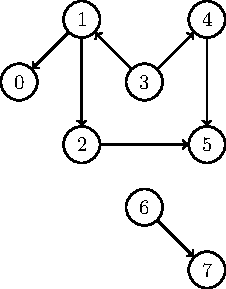
\includegraphics[scale=.8]{assets/chapter6/evaluateGraph.pdf}
    \caption{Visualisation of the graph data structure used to evaluate BST algorithms.}
    \label{evalGraph}
\end{figure}

\section{Presentable}

The last goal was that Psnodig should be presentable. We want to see if we can transpile the source programs we write to the presentation-only formats pseudocode and flowcharts.

\subsection{Pseudocode Writer}

The pseudocode writer aims to convert Psnodig ASTs to pseudocode. The writer gives us a LaTeX file by default, accompanied by the compiled result in a PDF if we wish. In this section, we will ignore the LaTeX files, and only look at the compiled versions. \\

The PDFs take up a considerable amount of space, so for readability reasons we will only present the ones relating to search algorithms. The rest will be located in \Cref{appendixB}.

\subsubsection{Search Algorithms}

\begin{figure}[ht!]
    \centering
    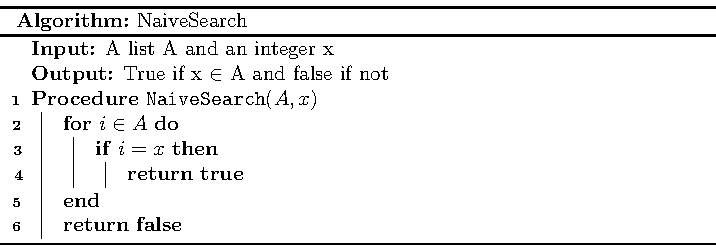
\includegraphics[scale=.8]{assets/chapter6/search/NaiveSearch_tbp.pdf}
    \caption{The result of transpiling \Cref{naiveSearchGourmet} to pseudocode.}
    \label{naiveSearchTBP}
\end{figure}

\begin{figure}[ht!]
    \centering
    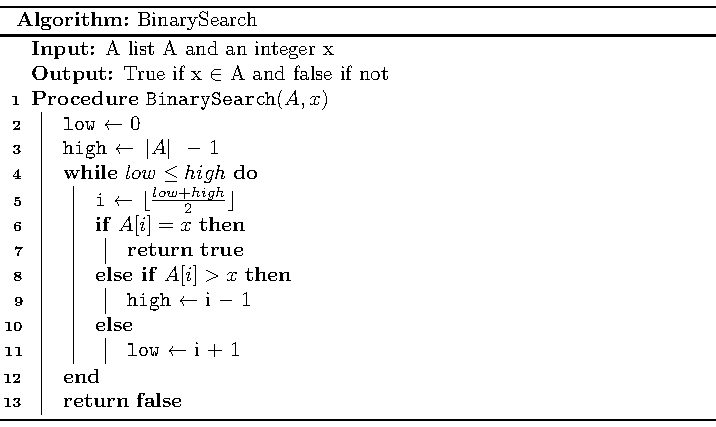
\includegraphics[scale=.8]{assets/chapter6/search/BinarySearch_tbp.pdf}
    \caption{The result of transpiling \Cref{binarySearchGourmet} to pseudocode.}
    \label{binarySearchTBP}
\end{figure}

\subsection{Flowchart Writer}

The flowchart writer is the most advanced of the four, working on yet another level of abstraction. The flowchart writer aims to convert Psnodig ASTs to flowcharts. Again, we receive a LaTeX file by default, but for the sake of evaluation we are only interested in the compiled results, ignoring the original LaTeX files. \\

As is the case with the TBP results, the IBP results span across a considerable amount of pages, and for readability reasons we will only present the ones relating to search algorithms. The rest will be located in \Cref{appendixC}.

\subsubsection{Search Algorithms}

\begin{figure}[ht!]
    \centering
    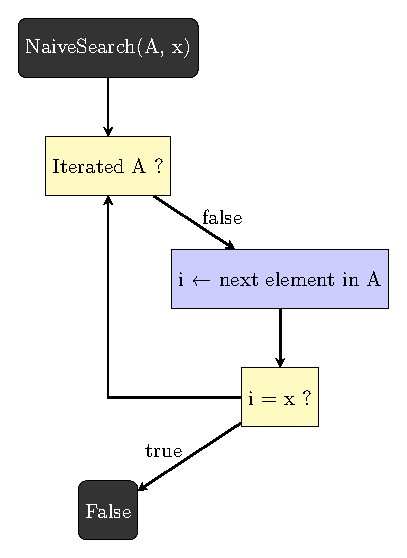
\includegraphics[scale=.7]{assets/chapter6/search/NaiveSearch_ibp.pdf}
    \caption{The result of transpiling \Cref{naiveSearchGourmet} to a flowchart.}
    \label{naiveSearchIBP}
\end{figure}

\begin{figure}[ht!]
    \centering
    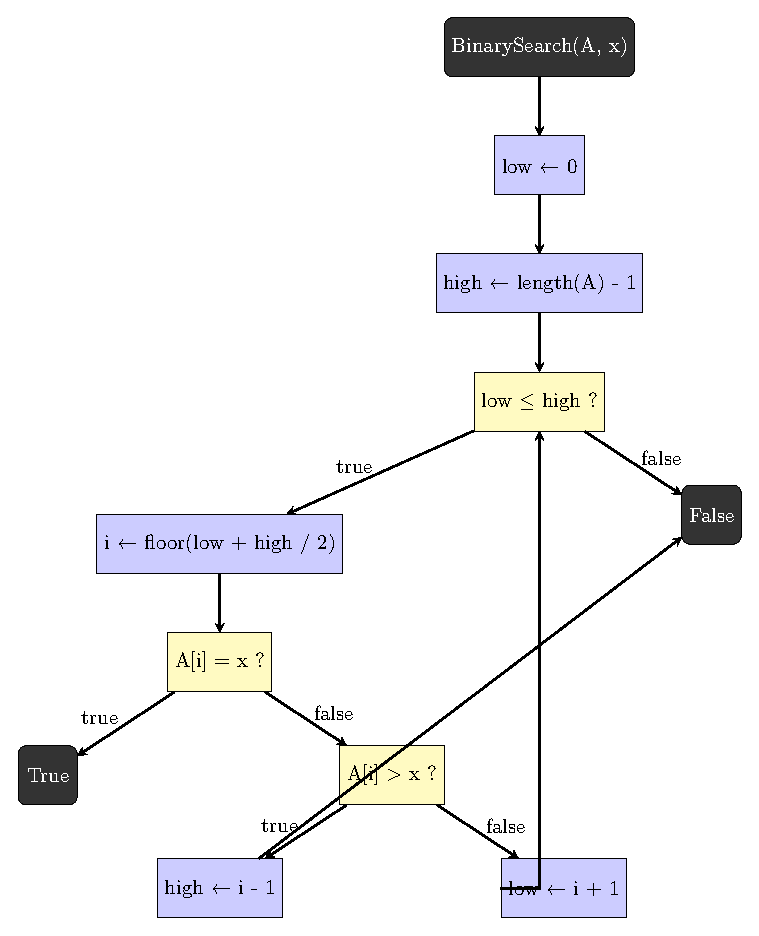
\includegraphics[scale=.65]{assets/chapter6/search/BinarySearch_ibp.pdf}
    \caption{The result of transpiling \Cref{binarySearchGourmet} to a flowchart.}
    \label{binarySearchIBP}
\end{figure}


\chapter{Discussion}

In this chapter, we discuss the results we obtained in Section 6.

\section{Reflections}

\subsection{Notation}

The TBP- and IBP writers work on a different abstraction level than those of Gourmet and Python. Where the two last ones are restricted to ASCII-based keywords like \texttt{!=} and \texttt{floor(x)}, the two first ones allow us to use more precise mathematical notation like \texttt{$\neq$} and \texttt{$\lfloor$x$\rfloor$}.

\subsection{Extensible}

We currently only have one parser, for the Gourmet programming language. However, we do believe that similar parsers could be added, without much extra work. The parser is currently 336 lines, and we have also preferred readability to conciseness, so we believe it could be done in even fewer. \\

\forsup{Oppdater dette tallet 14. mai!}

An additional point is that the parser clearly works, as discussed in Section 5.8.1, but it is also able to produce the computer programs we wanted to evaluate with ease. Given the general nature of Psnodig, we believe one could follow more or less the same steps that we have, to add a new parser.

\subsubsection{Adding writers}

\forsup{nei, ikke snakk om dette. men kanskje prøv å trekk en linje mellom str på gourmet parser og writer, og python writer, og si at det muligens kan være en liknende mengde jobb å legge til en parser (og parsere for liknende språk).}

\forsup{husk, gourmet- og python writer er egt ikke målet med thesisen. det er FRA soruce code TIL pseudokode og flytdiagram.}

Currently, Psnodig boasts four writers. Two of them are for programming languages, whilst the other two are presentation-only targets. \\

The Gourmet writer works, as we are able to losslessly transpile Gourmet code back to itself. We saw it in Section 6.1, and we were also able to run the transpiled versions and obtain the same results as we did with the original ones. The Gourmet writer spans 224 lines of code, showing the general effort of adding a writer. \\

The Python writer also works, as we are able to run the transpiled versions on the Python interpreter, and receive the same output as we did with Gourmet. The Python writer spans exactly 300 lines of code, showing the general effort of adding a writer for a subset of an existing language. \\

The two presentation-only writers both target LaTeX. Both are able to convert a Psnodig AST to LaTeX, despite the formats being somewhat different. Particularly the IBP writer works on a very different abstraction level, primarily consisting of nodes and edges. However, in the end it worked well, and the writers span 323 and 538 lines of code, respectively.

\subsection{Executable}

It is clearly executable.

\subsection{Does it hold up against the problem as a whole?}

We believe that Psnodig \textit{does} hold up against the problem definition introduced in Section 3.1, and that it successfully achieves the goals we set in Section 1.2. It is the first of its kind, a publically available tool that transpiles source code to TBP and IBP, as well as being executable, and is easy to add parsers and writers to.

\section{Limitations}

\subsection{Presentable}

% Complex flowcharts

We are able to successfully transpile all Psnodig data types to flowcharts on their own, and also construct more complex flowcharts, combining statements, expressions and more. \\

However, a limitation is that of nested control flow statements, being \texttt{While}, \texttt{For}, \texttt{ForEach}, and \texttt{If}. The biggest problem is that each edge has a fixed size, and when nesting these types of statements, we risk them crashing into each other. This can be seen in \Cref{deleteBSTIBP}, where one of the statements shadow parts of another. We also see, in \Cref{dfsIBP}, that edges sometime interfere with nodes, making it a bit difficult to know where they actually point.

\subsection{Extensible}

% Paradigm

Psnodig is primarily built to work with imperative languages, like Go and Python. This made it comfortable to write a parser for Gourmet, as well as the writers for Gourmet and Python. However, if the languages come from different paradigms, it might make it more challenging. \\

We believe it might be more challenging to add a parser for logic languages like Prolog, formal specification languages like TLA+, query languages like SQL etc. This is because they work in a different, and more specific way than general, imperative languages do. \\

It might also prove challenging to add a writer for these languages, especially if we are very dependent on structs or loops.

\forsup{Implementation language}

To add a parser or writer to Psnodig in the first place, they must be written in Haskell.\footnote{Technically, they can be written in a different language and \textit{transpiled} to Haskell.}

\subsection{Executable}

Doesn't capture infinite loops!

\chapter{Conclusion}

\forsup{Important: Remind the reader of all the good stuff!}

This section will give a summary of our contributions and discuss future work, before concluding the thesis.

\section{Future Work}

\subsection{Psnodig}

The syntax of Psnodig contains all the necessary building blocks to write complex computer programs, but as previously mentioned, the syntax shows the maximum available. Parsers and writers can easily utilise as little of the syntax as they want, for instance if we wish to create a simple calculator language. \\

Therefore, it could be interesting to expand Psnodig's syntax to include more things we commonly see today in programming, like lambda functions and more data structures. This would make the language even more flexible, and potentially make it more tempting for people to use.

\subsection{Interpreter}

The interpreter has its primary focus on correctness, and is not particularly optimised for speed. There are parts of the interpreter that could be optimised, utilising Haskell's features to a greater extent. For one, variable scopes are lists of \texttt{(String, Value)}-pairs, but the innermost layer could have been a mapping, which would shrink the ammortised runtime of lookups from $O(n)$ to $O(1)$. \\

Another flaw is that the interpreter will only stop on error or success. For instance, We do not have a way of identifying infinite loops by print statements like we can in many other language. This is because the print statements appear on the screen only when the program has terminated.

\subsection{Writers}

The writers all work in their own right, but there are always improvements to be made. This section covers what we believe to be the ones to make.

\subsubsection{Pytite Writer}

Currently, Pytite is a subset of Python, but we are not sure to what extent we cover the standard Python language. There are things we do not touch upon, like list comprehension, though there are patterns in the Psnodig syntax that could be recognised and converted accordingly.

\subsubsection{Pseudocode Writer}

We have utilised the Algorithm2e package, but there might be a different package we could use.

\subsubsection{Flowchart Writer}

As discussed in Section 7.2.1, the IBP writer struggles with complex flowcharts where we nest the statements types \texttt{While}, \texttt{For}, \texttt{ForEach}, and \texttt{If}. This could be improved by making the edges longer in these cases, or choosing different placement rather than always building flowcharts downwards.

\section{Summary of Contributions}

We introduced an imperative C-like programming language Gourmet, and the Python subset Pytite. \\

We designed a DSL Psnodig, and created an interpreter that runs on its internal representation. \\

We have added four writers to Psnodig, two of them being executable programming languages, and two of them being presentation-only targets.

\cleardoublepage
\addcontentsline{toc}{chapter}{\hspace{5mm}Bibliography}
\printbibliography

\end{document}
